% This thesis template is based on the personal template of Felix Moebius. Thanks, Felix!
% It has been extended and modified by Tobias Pfandzelter at the Scalable Software Systems group of TU Berlin.
% It is licensed under the terms of the MIT license, meaning you are free to use it however you see fit but we accept no liability.
% Good luck writing your thesis!

\documentclass[a4paper, 11pt]{article}

\usepackage[utf8x]{inputenc}
\usepackage[T1]{fontenc}
\usepackage{fix-cm}

\usepackage[a4paper, margin=3cm]{geometry}
\usepackage[titletoc, title]{appendix}

\usepackage{color}
\usepackage{booktabs}
\usepackage[all]{nowidow}
\usepackage[dvipsnames]{xcolor}
\usepackage[hidelinks]{hyperref}
\usepackage{acronym}
\usepackage{graphicx}
\usepackage{url}
\usepackage{titlesec}
\usepackage{csquotes}
\usepackage{amsmath}

\usepackage{transparent}
\usepackage{eso-pic}
\usepackage[section]{placeins}
\usepackage{setspace}
\usepackage{parskip}
\usepackage{subcaption}


%\renewcommand\thefigure{\thesection.\arabic{figure}} % Figures numbered as 5.1, 5.2, ...
%\renewcommand\thesubfigure{.\arabic{subfigure}} % Subfigures numbered as 1, 2, 3...
%\captionsetup[figure]{labelformat=simple, labelsep=period} % Ensures "5.1.1. Caption"
%\renewcommand\thefigure{%
%\thesection.\arabic{figure}}
%\renewcommand\thesubfigure{%
%\thesection.\arabic{figure}.\arabic{subfigure}}
\renewcommand\thetable{%
\thesection.\arabic{table}}

\usepackage[main=english, ngerman]{babel}

% we use the cleveref package to refer to figures, sections, etc.
% instead of "Figure~\ref{fig:example}", write only "\cref{fig:example}" and the word "Figure" (or table, etc) will be inserted normally
\usepackage[noabbrev,capitalise]{cleveref}

\usepackage[
    maxbibnames=99,
    style=numeric,
    url=false,
    backend=bibtex8,
    sortcites=true,
]{biblatex}
\addbibresource{refs.bib}
\DeclareFieldFormat[online]{urldate}{Last accessed: #1}
\DeclareFieldFormat{eprint}{arXiv: \href{https://arxiv.org/abs/#1}{#1}}
\DeclareFieldFormat[report]{title}{``#1''}


\newcommand{\projectTitle}{Performance Prediction in Application Benchmarks using Microbenchmarks}
\newcommand{\thesisType}{Master's Thesis}
\newcommand{\authors}{Daniel Klinkert Houfer}
\newcommand{\matrikel}{451761}
\newcommand{\authorEmail}{\href{mailto:daniel.klinkerthoufer@campus.tu-berlin.de}{daniel.klinkerthoufer@campus.tu-berlin.de}}
\newcommand{\examinera}{Prof.~Dr.-Ing.~David Bermbach}
\newcommand{\examinerb}{Prof.~Dr.~habil.~Odej Kao}
\newcommand{\supervisor}{Nils Japke}

\newcommand{\projectYear}{2025}
\newcommand{\facultyName}{Fakultät Elektrotechnik und Informatik}
\newcommand{\departmentName}{Fachgebiet Scalable Software Systems}

\begin{document}
{\sffamily\color{white}\raggedright\setlength{\parindent}{0cm}\large\onehalfspacing
\AddToShipoutPicture*{
    \put(-4,0){
        \parbox[b][\paperheight]{\paperwidth}{%
            \vfill
            \centering
            
\includegraphics[width=\paperwidth]{title.pdf}%
            \vfill
        }
    }
}

\vfill
\vspace*{5cm}

{\huge\textbf{\projectTitle}\par}
\vspace*{0.5cm}
\textbf{\thesisType}      \\
\vspace*{2cm}
\textbf{Author}               \\
\authors              \\
\matrikel                     \\
\authorEmail                  \\
\vspace*{1cm}
\textbf{Advisor}              \\
\supervisor                   \\
\vspace*{1cm}
\textbf{Examiners}            \\
\examinera                    \\
\examinerb

\vfill

\textbf{Technische Universit\"at Berlin, \projectYear} \\
\small{\facultyName \\
    \departmentName}
\vspace{1cm}
}

\thispagestyle{empty}
\clearpage

\vspace*{\fill}
\begin{centering}
    {\huge\textbf{\projectTitle}\par}
    \vspace{1cm}
    \large{\thesisType}\\
    \vspace{1cm}
    Submitted by:\\
    \authors\\
    \matrikel                     \\
    \authorEmail                  \\
    \vspace{1cm}
    Technische Universit\"at Berlin\\
    \facultyName \\
    \departmentName \\
    \vspace{1cm}
    \projectYear\\

\end{centering}

\vspace*{\fill}
\thispagestyle{empty}
\clearpage

\vspace*{\fill}
{
    % briefly set the footnote to symbols for this disclaimer
    \renewcommand*{\thefootnote}{\fnsymbol{footnote}}
    \noindent
    \begin{otherlanguage}
        {ngerman}
        Hiermit versichere ich, dass ich die vorliegende Arbeit eigenständig ohne Hilfe Dritter und ausschließlich unter Verwendung der aufgeführten Quellen und Hilfsmittel angefertigt habe.
        Alle Stellen die den benutzten Quellen und Hilfsmitteln unverändert oder sinngemäß entnommen sind, habe ich als solche kenntlich gemacht.

        Sofern generische KI-Tools verwendet wurden, habe ich Produktnamen, Hersteller, die jeweils verwendete Softwareversion und die jeweiligen Einsatzzwecke (z.~B.~sprachliche Überprüfung und Verbesserung der Texte, systematische Recherche) benannt.
        Ich verantworte die Auswahl, die Übernahme und sämtliche Ergebnisse des von mir verwendeten KI-generierten Outputs vollumfänglich selbst.

        Die Satzung zur Sicherung guter wissenschaftlicher Praxis an der TU Berlin vom 8. März 2017\footnote{\url{https://www.static.tu.berlin/fileadmin/www/10000060/FSC/Promotion___Habilitation/Dokumente/Grundsaetze_gute_wissenschaftliche_Praxis_2017.pdf}} habe ich zur Kenntnis genommen.

        Ich erkläre weiterhin, dass ich die Arbeit in gleicher oder ähnlicher Form noch keiner anderen Prüfungsbehörde vorgelegt habe.
        \vskip 2cm
        \begin{tabular}{@{}p{.5in}p{4in}@{}}
             & \hrulefill                              \\
             & (Unterschrift) \authors, Berlin, \today \\
        \end{tabular}

    \end{otherlanguage}
    % reset footnote styling for the rest of the thesis
    \renewcommand*{\thefootnote}{\arabic{footnote}}
    \setcounter{footnote}{0}
}

\vspace*{\fill}
\thispagestyle{empty}
\clearpage

\newpage

\section*{Abstract}

Performance testing is gaining more focus in modern software development nowadays, ensuring that applications meet efficiency and scalability goals. There are two standard practices: application benchmarks and microbenchmarks. Application benchmarks test an entire application under realistic conditions and require substantial time and resources. On the other hand, microbenchmarks measure the performance of specific functions or components. This thesis investigates how microbenchmark results can accurately predict or correlate with full-scale application performance in a cloud environment.
Using VictoriaMetrics as the system under test \ac{SUT}, we conducted application benchmarks using the Time Series Benchmark Suite \ac{TSBS} and microbenchmarks with an adapted \ac{GoAbs} framework. To mitigate noise from shared cloud resources, we applied techniques such as duet benchmarking for application tests and Randomized Multiple Interleaved Trials \ac{RMIT} for microbenchmarks. Through a ridge regression model we then examined whether microbechmarks execution times could be linked to application-level latencies, assessing whether isolated function performance changes reliably reflect end-to-end behavior. Our findings show that microbenchmarks provide valuable insights into function-specific performance. However, their direct predictive power over application benchmarks remains limited—especially under a purely linear modeling approach and high collinearity among the microbenchmark functions. This research concludes that without more advanced modeling or supplementary validation, microbenchmarks alone may not sufficiently be able to predict performance improvements or regressions on the application benchmark level. Therefore, improvements and further work for benchmarking practices are discussed, including expanded feature selection techniques and non-mean metrics, and directions for future research into correlating micro- and application-level performance are proposed.


% GERMAN
\clearpage
\begin{otherlanguage}
    {ngerman}
    \section*{Kurzfassung}
    In der modernen Softwareentwicklung spielt Performance Testing eine zunehmend zentrale Rolle, dabei soll sichergestellt werden, dass Anwendungen die Anforderungen an Effizienz und Skalierbarkeit erfüllen. Dafür kommen vor allem zwei Methoden zum Einsatz: Application Benchmarks, bei denen ein gesamtes System unter realitätsnahen Bedingungen getestet wird und die daher umfangreiche Zeit und Ressourcen beanspruchen, sowie Microbenchmarks, die gezielt die Performance einzelner Funktionen oder Komponenten untersuchen.
    Diese Masterarbeit geht der Frage nach, inwieweit sich aus Microbenchmark-Ergebnissen belastbare Vorhersagen über die Gesamtleistung einer Anwendung in einer Cloud-Umgebung ableiten lassen. Hierzu wird VictoriaMetrics als System under Test \ac{SUT} verwendet, haben wir application benchmarks mit der Time Series Benchmark Suite \ac{TSBS} durchgeführt. Parallel haben wir Microbenchmarks mit einem angepassten \ac{GoAbs} Framework ausgeführt. Um störende Einflüsse geteilte Cloud-Ressourcen zu reduzieren, kam dabei Duet-Benchmarking (für die Anwendungstests) und Randomized Multiple Interleaved Trials \ac{RMIT} (für die Microbenchmarks) zum Einsatz. Anschließend wurden die Ausführungszeiten der Microbenchmarks mittels Ridge-Regression mit den Latenzen auf Anwendungs-Ebene vergleichen, ob sich Veränderungen in der Leistung einzelner Funktionen zuverlässig auf das Gesamtsystem übertragen lassen. Unsere Resultate zeigen, dass Microbenchmarks zwar wertvolle Einblicke in die Leistungsfähigkeit spezifischer Funktionsbereiche liefern, ihre direkte Vorhersagekraft für vollständige Anwendungs-Benchmarks jedoch begrenzt ist—insbesondere bei rein linearen Modellierungsansätzen und hoher Korrelation zwischen den einzelnen Microbenchmark-Funktionen. Wir schließen daraus, dass Microbenchmarks ohne weiterführende Modellierung oder ergänzende Validierung nur eingeschränkt in der Lage sind, Verbesserungen oder Verschlechterungen auf Anwendungsebene präzise vorherzusagen. Deshalb werden mögliche Verbesserungsmaßnahmen diskutiert, darunter erweiterte Verfahren zur Merkmalsauswahl, sowie nicht-lineare Metriken. Abschließend werden Perspektiven für künftige Forschung aufgezeigt, die darauf abzielen, das Zusammenspiel von Micro- und Anwendungs-Performance noch fundierter zu erschließen.
\end{otherlanguage}

\clearpage
\tableofcontents
\clearpage
\listoffigures

\clearpage
\listoftables

\clearpage
\section*{Abbreviations}
\begin{acronym}
    \acro{SUT}[SUT]{System under test}
    \acro{TSBS}[TSBS]{Time Series Benchmark Suites}
    \acro{GoAbs}[GoAbs]{Go API Benchmarking Score}
    \acro{RMIT}[RMIT]{Randomized multiple interleaved trials}
    \acro{CI}[CI]{Continuous integration}
    \acro{CD}[CD]{Continuous deployment}
    \acro{VM}[VM]{Virtual Machine}
    \acro{ms}[ms]{Milliseconds}
    \acro{MSE}[MSE]{Mean Squared Error}
    \acro{VIF}[VIF]{Variance Inflation Factor}
    \acro{PCA}[PCA]{Principal Component Analysis}
    \acro{TCP}[TCP]{Test Case Prioritization}
    \acro{API}[API]{Application Programming Interface}
    \acro{I/O}[I/O]{Inpout/Output}
    \acro{CPU}[CPU]{Central processing unit}
    \acro{RAM}[RAM]{Random access memory}
\end{acronym}

\clearpage
\section{Introduction}
\label{cha:introduction}

Modern development practices no longer focus solely on testing and ensuring the application's functionality. There is a growing emphasis and interest in evaluating and measuring applications’ performance to gain deeper insights into their efficiency, responsiveness, and reliability \cite{chen2017exploratory, ameller2012software}. By analyzing performance, developers can understand how users interact with applications, make data-driven decisions, and optimize resource usage \cite{chen2017exploratory, bulej2019initial, gunningberg1989application, ameller2012software}. \\ 
There are three main ways to characterize an application’s performance: latency, scalability, and throughput \cite{denaro2004early, laaber2019continuous}. Research defines latency as the delay between the operation and the executed action \cite{dimitrov2000impact, denaro2004early}. Scalability refers to the dependency between the number of resources a system can handle without excessive additional costs \cite{denaro2004early, bondi2000characteristics}. Lastly, research describes throughput as the response rate of the number of actions and operations that can be completed under a certain period \cite{r2006throughput, denaro2004early}. Any change in any of them may result in a performance issue that affects the application’s overall behavior.  \\
Performance is an issue that can affect both developers and the end user, affecting customer satisfaction and determining the application’s success. On the one hand, it affects end users given the fact that performance issues affect the overall behavior of the application and tend to have a significant impact on user experience, driving users away, discouraging engagement, decreasing the application’s responsiveness, and undermining the application’s reputation \cite{grambow, alghamdi2023towards}. On the other hand, for developers, these issues are more than just inconveniences or bugs; they represent costs, time investment, and potential delays in upcoming releases.  \\
Developers detect performance issues as either performance bugs or regressions. Its early detection reduces and mitigates escalating problems that can impact the application more. Performance bugs refer to programming errors that cause inefficient application operation and tend to create functional bugs and crashes \cite{nistor2013discovering}. Developers tend to see these bugs when a new feature is implemented for the first time, affecting the application’s overall performance. Usually, performance bugs tend to require more time and more experienced developers to fix them; hence, they require more resource utilization and higher costs \cite{bermbach2017quality}. Performance regressions mean that even if the performance of the application is meeting the requirements, it is lower than its previous version that previously performed well; for example, an update or a code change can lead to having a lower time response than before, or there is an increase of resource utilization \cite{nguyen2014industrial}. Both performance bugs and regressions can highly impact the application’s user experience and interaction; therefore, developers must address performance issues early in the development cycle \cite{chen2017exploratory, foo2010mining}. If developers detect a performance bug or regression late, the costs, resources, and efforts required to fix it are higher \cite{grambow2021usingApplication}. For this reason, proactively identifying and solving these issues early enough avoids bigger failures, costs, and waste of resources and reduces long-term maintenance costs by preventing future failures in production \cite{nistor2013discovering, shang2015automatedDetection}. \\
Ali et al. \cite{ali2022performance} argue that testing ensures quality and control throughout development. Nowadays, performance issues can be proactively detected when properly testing the application’s performance before deployment. Developers can perform specific tests to measure performance and identify and resolve issues during the development cycle \cite{ali2022performance}. A performance test mimics the actual application’s performance in a real-case scenario, with underlying potential problems, to solve them before deploying an application; it aims to validate the \ac{SUT} reliability and stability \cite{ali2022performance}. Performance tests enable developers to make the necessary changes without harming the application’s behavior and overall performance. Thus, end-users will not be affected \cite{alghmadi2016automated, chen2017exploratory, foo2010mining}. In this way, performance testing helps detect if any committed code changes may have affected the application’s performance and evolution before releasing a new version of the system \cite{alshoaibi2019DetectionofPerformance, shang2015automatedDetection}.  \\
One of the most common methods of measuring an application’s performance is benchmark suites, a set of standardized tests designed to measure the performance of a system under various conditions \cite{alghamdi2023towards}. The benchmark suites’ objective is to assess an application’s performance under different workloads and conditions, ensuring it meets the performance requirements \cite{alghamdi2023towards, japke2023earlymicrobenchmarkcatches}.These suites aim to stress a system under test, further referred to as \ac{SUT}, with artificial loads that are as real as possible to a real scenario while observing its response using quality metrics, comparing the results with another system or even a previous version to detect performance changes early in time to avoid bigger failures \cite{alghamdi2023towards, japke2023earlymicrobenchmarkcatches, grambow, grambow2021usingApplication, varghese2021survey, folkerts2012benchmarking}. Nowadays, benchmarks are used throughout the different phases of an application life cycle. They are commonly used in the application’s development, implementation, and maintenance to test performance changes \cite{tsuji2017performanceprojection} and deployment. \\
Benchmark suites help developers mitigate the unpredictability of the cloud infrastructure, allowing them to perform repeatable tests in a controlled scenario \cite{japke2023earlymicrobenchmarkcatches}. Although running benchmarks after every code change will enable developers to identify potential performance issues quickly, it is not feasible due to the time it takes to run the performance benchmarks and the associated costs \cite{grambow, alshoaibi2019DetectionofPerformance, he2019statistics}. On top of that, it also delays further application development as developers will need to wait for the results of every benchmark suite to detect a performance change, which increases the amount of required resources like time, costs, and infrastructure \cite{alshoaibi2019DetectionofPerformance, grambow, grambow2021usingApplication, he2019statistics}. The developer is responsible for identifying the best and optimal time to run the benchmarks to obtain meaningful results while balancing efficiency and effectiveness \cite{de2017perphecyperformance}. The benchmark results help developers identify bottlenecks or the root cause of problems, enabling them to evaluate and optimize changes to boost the application’s performance while minimizing resource use and costs \cite{alshoaibi2019DetectionofPerformance, he2019statistics}. Moreover, it gives developers insights into the performance data to make well-informed decisions. \\
Cloud computing has revolutionized how we currently deploy and test applications. The aim is to provide a familiar and integrated platform that multiple users can use simultaneously \cite{hwang2015cloudperformance}. Its infrastructure as a service model and its variety of cloud services have made it popular for performance testing \cite{scheuner2018cloudBenchmarkingSuit, scheuner2018estimatingCloudApplication}. Cloud environments offer flexibility, scalability, reduced infrastructure costs, and simplified maintenance, making them attractive for performance testing. They provide all its resources, such as storage, computing, and networking over the internet \cite{vazquez2014cloudBenchmarkSurvey, borhani2014wpress, langer2011virtualmachineperformancebenchmarking}. It is composed of virtual machines that offer several resources like memory, storage, \ac{CPU}, machine architecture, and \ac{I/O} performance to its users \cite{gillam2013fair}. Given that these resources are available, it is no longer necessary to run the applications in bare metal hardware; instead, they can be deployed in the cloud \cite{he2019statistics, iosup2011performanceVariability}. Thus, cloud computing reduces the need for companies to keep and maintain expensive computing hardware \cite{iosup2011performanceVariability}. Nonetheless, not everything is perfect when deploying to cloud environments. Cloud computing provides unlimited resources for users to generate tests and run simulations. However, using those resources carefully and efficiently is still necessary to reduce costs when performing tests \cite{snellman2011towardsAutomatic}. \\
Furthermore, cloud environments can offer a wide variety of virtual machines (\ac{VM}), and each of them meets different requirements and trade-offs for applications \cite{scheuner2018estimatingCloudApplication, varghese2016cloudbenchmarkingformaximising}. Thus, developers must choose the best \ac{VM} that maximizes their application and performance goals \cite{yadwadkar2017selectingthebest, varghese2016cloudbenchmarkingformaximising}. It is essential to consider that in cloud environments, developers lower the control they have over the software, and they can have shared hardware between different cloud consumers, leading to their application not having access to the complete resources of the virtual machine, affecting the measurements of performance by making it challenging to detect accurate results \cite{he2019statistics, laaber2019softwaremicrobenchmarkinginthecloud, xiong2013Anautomatedmodeldrivenframework} and scale to meet the end-users requests \cite{vazquez2014cloudBenchmarkSurvey, folkerts2012benchmarking}. \\
Therefore, testing that covers uncertain factors is required to provide accurate performance results \cite{he2019statistics}. Benchmarking the performance multiple times and for extended periods is necessary so that the findings do not rely on a single instance and the outcomes can be perceived throughout the experiment. However, limitations have to be considered, as there is a trade-off between costs and execution time \cite{bulej2019initial, laaber2021applyingtcp, mostafa2017perfrankerprioritization}. This trade-off is one of the biggest challenges when addressing performance issues, as developers do not know precisely how long a performance test has to be run to detect issues or changes in its performance \cite{alghmadi2016automated, alghamdi2023towards}. Hence, having a short execution time might result in fewer costs but might lead to underperformance and inaccuracy in the performance metrics collected. However, extending the testing time might produce more accurate results. Still, it comes at the expense of higher costs and computer resources\cite{alghamdi2023towards, he2019statistics, bulej2019initial, bulej2020duet, grambow2020benchmarkingMicroservicesperformance, laaber2021applyingtcp}. For this reason, developers need to be careful when deciding the most cost-effective solution and how long they want to run the experiments to get the best estimation of how performant the software will be so they can minimize unnecessary costs and waste of resources while still offering reliable insights into the performance of the application to make data-driven decisions, updates or changes in the application. \\
Developers have two benchmarking options for measuring and testing an application’s performance: microbenchmarks and application benchmarks. Microbenchmarks test specific function’s performance and must be run repeatedly. As microbenchmarks are very specific and focus only on a particular function, it is hard to know whether a change in this benchmark will impact the overall application’s performance in the real world \cite{bulej2019initial, grambow, laaber2022multi}. On the other hand, an application benchmark is more robust and complex than microbenchmarks since it needs to bring up the whole application into a testable state, which adds much complexity considering multiple factors such as machine configuration, hardware, and network \cite{japke2023earlymicrobenchmarkcatches}.Therefore, running the application benchmark as often as every commit would not be feasible due to the long runtimes, multiple repetitions, resources, and costs it conveys \cite{grambow, japke2023earlymicrobenchmarkcatches, bulej2019initial}. Together, microbenchmarks and application benchmarks enable developers to design, test, and optimize applications in the cloud to detect issues in advance and maximize their performance and reliability. In their paper, Grambow et al. \cite{grambow} stated that detecting an application’s performance is possible using microbenchmark suites. Hence, after considering this study, this thesis aims to establish a correlation between the performance change detected in a microbenchmark and its impact on the application’s benchmark performance using another method. \\
This thesis research question is to what extent can the microbenchmarks predict a slow-down in the application benchmarks’ performance? By doing so, it seeks to enable developers to use microbenchmark results as early indicators of broader performance trends, applying different methodologies that will lead to reality results. The motivation behind this project is to develop a stable and well-proven correlation between the microbenchmark results and application benchmark that saves time and decreases the number of non-performant production releases, giving developers early feedback on the performance changes. 
\clearpage
\section{Background}
\label{cha:background}
Cloud benchmarking is a common way to study and analyze the quality and performance of cloud services based on experiments  \cite{bermbach2017quality, vazquez2014cloudBenchmarkSurvey}. However, every cloud environment has constraints such as shared resources among users, high costs, and a wide variety of Virtual Machines \cite{snellman2011towardsAutomatic, scheuner2018estimatingCloudApplication}. Despite these constraints, it can be effectively used by using benchmarking tools that create artificial workloads to measure its quality and collect information on states \cite{grambow2020benchmarkingMicroservicesApplication, grambow2019continuousBenchmarking, bermbach2017quality}. \\
Benchmarking aims to answer specific questions and compares different software versions, deployments, and configurations to report and evaluate how well a system under test can handle specific and predefined workloads under specific resource constraints. It aims to retrieve accurate and meaningful results to assess a system’s performance and reduce the uncertainty in a production release \cite{folkerts2012benchmarking, grambow2020benchmarkingMicroservicesApplication, grambow2019continuousBenchmarking, grambow2020benchmarkingMicroservicesperformance}. \\
Its objective is to offer developers a solution to compare the results of running different scenarios under the same conditions in a structured, repeatable, and measurable way to identify and evaluate performance changes and optimize them accordingly before deploying an application and consuming cloud resources \cite{shang2015automatedDetection}. \\
This method gives developers a detailed breakdown of how the application’s behavior will be under scenarios similar to those encountered after deployment \cite{palit2016demystifying, palit2016demystifying}. Additionally, benchmarking can simulate scenarios under extreme conditions to uncover potential failures before they manifest in production, reducing downtime, ensuring a smoother user experience, minimizing costs, and ensuring scalability \cite{japke2023earlymicrobenchmarkcatches, grambow2020benchmarkingMicroservicesperformance, grambow2020benchmarkingMicroservicesApplication}. However, benchmarking can be costly. To mitigate costs, the developer should constantly monitor and analyze the results to identify if the requirements have been met \cite{grambow2020benchmarkingMicroservicesperformance}. \\
There are two main benchmarking techniques: application benchmarks and microbenchmarks. Although they are different techniques, they share the same general objective: to identify and test the performance of an environment using a system under test to simulate realistic workloads and real-world usage \cite{japke2023earlymicrobenchmarkcatches, grambow2021usingApplication, grambow2020benchmarkingMicroservicesperformance}. These techniques help developers understand how the system will behave under typical or extreme conditions, allowing them to rely on quantifiable and insightful data to assess its capabilities and enhance their decision-making. 

\subsection{Application Benchmark}
\label{sec:application_benchmarks}
This benchmarking technique tests the entire system. It deploys the \ac{SUT} into an environment similar to production by generating artificial loads into the system to simulate real-world conditions. It evaluates how the application behaves under an established atmosphere by measuring response time, throughput, and scalability \cite{denaro2004early}. Application benchmarks are often preferred when the goal is to understand how well a cloud platform supports the application's performance \cite{grambow2021usingApplication}. A client generally generates the load of the application's benchmark to avoid using the \ac{SUT}'s resources to develop fake loads; therefore, the \ac{SUT} is like a black box where only its \ac{API}s are used to stress the system \cite{japke2023earlymicrobenchmarkcatches}. It aims to help developers understand and evaluate the application's performance under expected stress scenarios and how well the system under test can handle artificial workloads. \\
However, replicating a complete production environment for application benchmarking is complex and time-consuming. Developers may face several challenges when doing application benchmarks. On the one hand, they must make critical decisions in advance, including selecting the appropriate machine configuration, network setup, and storage capacity. These decisions will impact the accuracy of the results. Additionally, multiple external factors can affect the performance of the \ac{SUT} when running the application benchmark on the cloud \cite{denaro2004early}. As Bulej et al. \cite{bulej2019initial} stated, the resources in the cloud could be shared between multiple applications, affecting the \ac{SUT}'s available resources. Similarly, depending on the machine type, the cloud provider might boost the machine's performance, affecting the end measurable results, which can introduce variability in the results and make it challenging to obtain consistent, reliable, and repeatable performance data. Therefore, as Grambow et al. \cite{grambow} stated, running this benchmark multiple times is recommended to obtain meaningful resources, leading to higher costs and the use of computer resources. To address these challenges, developers tend to implement techniques like duet benchmarking, which reduces the impact of external noise in shared environments by ensuring that performance results are not affected by these external factors \cite{bulej2020duet}.

\subsubsection{Duet Benchmarking}
\label{sec:duet_benchmarking}
As previously stated, the client executes artificial workloads in a shared cloud environment. This shared environment often leads to performance variability caused by external noise, which refers to any factor or situation outside the system under test that can affect or influence its performance, which might affect the benchmark’s overall performance \cite{japke2023earlymicrobenchmarkcatches, bulej2020duet}. \\
Bulej et al. \cite{bulej2019initial} argue in their research that duet benchmarking is a recommended technique to address this challenge, as external noise can compromise the reliability and accuracy of benchmark results. \\
Duet benchmarking measures the results obtained by two workloads executed in parallel in the same virtual machine. Both workloads are exposed to the same external factors since they share the same computational environment and resources \cite{bulej2019initial, bulej2020duet, grambow}. Duet benchmarking guarantees that any external influences, for example, other workloads that affect the cloud or shared resources, will have an equal impact on both workloads instead of only one; thus, making a fair comparison of the performance results of the workloads and the same result should be obtained \cite{bulej2019initial, bulej2020duet}. \\
The key feature of duet benchmarking is its ability to neutralize and reduce the impact of external factors on performance assessment \cite{bulej2019initial}. Since both workloads experience the same conditions, any observed differences in performance can be attributed directly to the system under test rather than the environmental noise, making performance results more accurate and reliable \cite{bulej2019initial, bulej2020duet}. Moreover, duet benchmarking helps developers identify and highlight meaningful differences between the compared workloads. Since both workloads operate under identical conditions, the technique effectively isolates performance changes related to the system rather than external factors, ensuring that these differences are evaluated under the same consistent and realistic operating conditions \cite{bulej2020duet}. Therefore, this technique provides a more precise assessment of the \ac{SUT} performance improvements or regressions, preventing developers from being misled by external noise \cite{japke2023earlymicrobenchmarkcatches}. \\
Lastly, this technique prevents developers from being misled by external noise by reducing bias by standardizing the testing environment for both workloads; duet benchmarking ensures consistent and realistic operating conditions. This consistency reduces the variability in results, enabling developers to trust the performance data and make informed decisions about optimizing the application \cite{bulej2020duet, bulej2019initial, japke2023earlymicrobenchmarkcatches}.

\subsection{Microbenchmark}
\label{sec:microbenchmark}
Opposite to application benchmarks, which focus on evaluating the entire system's performance under real-world scenarios, microbenchmarks focus only on testing individual and specific functions of the \ac{SUT} without considering the context of the entire application \cite{gil2011microbenchmarkleasonslearned, laaber2019continuous}. These microbenchmarks evaluate the \ac{SUT} by repeatedly calling the particular function under test with artificial workloads for a specific duration and number of iterations \cite{japke2023earlymicrobenchmarkcatches, grambow, laaber2019softwaremicrobenchmarkinginthecloud, bermbach2017benchfoundry}. This specific scope allows microbenchmarks to provide detailed insights into what is happening with the performance behavior in specific functions of the system under test. However, as Gil et al. \cite{gil2011microbenchmarkleasonslearned} argued, developers can draw wrong or inconclusive conclusions from the experiment if a microbenchmark suite is not executed correctly using the appropriate functions.  \\
Microbenchmarks detect performance issues on specific functions and resources. They allow developers to debug performance bottlenecks by evaluating code changes' impact on an isolated function without considering the external environment or the entire application \cite{scheuner2018estimatingCloudApplication, seltzer1999thecaseforapplicationspecific}. Therefore, microbenchmarks help understand the raw capabilities of specific resources or functions by measuring how the system will react to small workloads when testing isolated features \cite{bermbach2017benchfoundry, gil2011microbenchmarkleasonslearned}. \\
Microbenchmarks serve as the building blocks for predicting the behavior and performance of the entire application \cite{grambow}. Moreover, microbenchmarks allow developers to isolate components and fine-tune them, improving their functionalities and mitigating poor performance that could impact the entire application’s behavior. This predictive power gives developers confidence in their testing strategies and the ability to address potential performance issues \cite{scheuner2018estimatingCloudApplication, grambow2021usingApplication} proactively.\\
Microbenchmarks are relatively more straightforward than application benchmarks as they require a minimal setup \cite{japke2023earlymicrobenchmarkcatches}. Therefore, they take less time to set up and execute, making them less resource-intensive and faster to run \cite{grambow}. Since they are easier to set up than application benchmarks, developers tend to include them more often in the \ac{CI}/\ac{CD} pipelines to measure and provide insights on performance metrics such as \ac{CPU} usage, I/O throughput, latency memory consumption, execution time, storage, and network performance \cite{scheuner2018cloudBenchmarkingSuit, laaber2024evaluatingSeachbasedsoftware, grambow2021usingApplication, scheuner2018estimatingCloudApplication, laaber2021applyingtcp, sun2022dissecting}. \\
Frequent testing helps developers get faster warnings on how the function behaves without waiting for the whole application to be deployed. Additionally, running microbenchmarks often and throughout the development process leads developers to identify performance issues and bottlenecks early \cite{schirmer2024elastibench}. However, given that a \ac{SUT} has multiple functions when designing a microbenchmark suite, it is required to determine and carefully select which functions to benchmark to avoid redundancy and ensure resource allocation and reliable results. As Scheuner and Leitner \cite{scheuner2018cloudBenchmarkingSuit} argues, a prior benchmark selection helps avoid running similar microbenchmarks that will bring similar results and avoid undesirable testing, ensuring more efficient use and allocation of resources. Not having this prior careful selection can lead developers to run similar microbenchmarks that lead to undesirable duplicating results that provide unreliable insights about the function's performance, leading to poor testing practices and waste of resources. \\
Similarly to application benchmarks, running multiple microbenchmarks from the same suite is recommended to increase the likelihood of getting reliable results \cite{gil2011microbenchmarkleasonslearned}. However, despite their result precision, microbenchmarks face a limitation. Since the microbenchmarks' scope is limited, similar to unit tests, it is hard to know if the outcome of the microbenchmarks will have a real improvement or downgrade in the performance of the production environment. They might not reflect the impact in the whole tested environment, given that they solely focus on isolated functions while ignoring other parts of the application \cite{grambow, grambow2021usingApplication}. \\
In their research, Scheuner and Leitner \cite{scheuner2018cloudBenchmarkingSuit} suggest implementing different techniques to get more accurate results and reduce bias when making microbenchmarks. One of the most common techniques is randomized multiple interleaved trials, further referred to as \ac{RMIT}, which shuffles the execution order of workloads across iterations  \cite{japke2023earlymicrobenchmarkcatches, scheuner2018cloudBenchmarkingSuit}. This technique decreases the probability of having the same results by running the same artificial workloads in the same way all the time \cite{abedi2017conductingrepeatable}. By introducing randomness, \ac{RMIT} enhances the reliability of microbenchmark results and ensures that the insights obtained on the isolated functions are robust and actionable. 

\subsubsection{Randomized Multiple Interleaved Trials}
\label{sec:randomizedMultipleInterleavedTrials}
Considering the best practices for getting more accurate and unbiased results and avoiding the SUT of expecting a specific workload order, Scheuner and Leitner \cite{scheuner2018cloudBenchmarkingSuit} recommend in their research that microbenchmark suites be tested using Randomized Multiple Interleaved Trials (\ac{RMIT}). This technique addresses potential biases by avoiding predictable execution orders in the SUT, ensuring the performance measures are reliable and stable \cite{scheuner2018cloudBenchmarkingSuit, abedi2017conductingrepeatable}. It runs the microbenchmarks multiple times on the same cloud \ac{VM}s, shuffling their execution order each time by reorganizing the test's order and repeating the execution of the microbenchmark suite multiple times while keeping them as realistic an environment as possible, reducing the influence of external noise  \cite{japke2023earlymicrobenchmarkcatches,scheuner2018cloudBenchmarkingSuit}, while ensuring that the runs are not affected by the environmental changes \cite{abedi2017conductingrepeatable}. \\
Shuffling the artificial workloads in every iteration prevents the system under test from adapting or learning specific patterns of the instances, which could lead to unreliable results \cite{abedi2017conductingrepeatable, scheuner2018cloudBenchmarkingSuit}. Furthermore, this technique ensures that performance measurements remain reliable, even in dynamic and non-controlled environments \cite{abedi2017conductingrepeatable, scheuner2018cloudBenchmarkingSuit}. However, even though it reduces bias and ensures more accurate performance measurement, this technique has a limitation as it increases the execution time of the experiment, leading to more usage of resources, time, and costs  \cite{japke2023earlymicrobenchmarkcatches}. \\
The main advantage of \ac{RMIT} is its ability to mitigate the effects of unpredictable factors that might affect the microbenchmark's performance measurements. These factors are external sources that developers cannot control; the most common are resource and infrastructure fluctuations \cite{abedi2017conductingrepeatable}. To deal with these factors \ac{RMIT} distributes the impact of these external influences across a broader dataset by randomizing workload execution and conducting multiple trials, reducing their impact and influence in the final results \cite{abedi2017conductingrepeatable}. This randomization enables developers to fairly compare the results obtained in the microbenchmark and reduce bias, decreasing the probability of the same instance getting affected by external noise every time it runs. Therefore, \ac{RMIT} helps developers mitigate these external influences, providing a more robust, reliable, and unbiased performance measure while ensuring that the results will be based on a real-case scenario and not on a single instance. Thus, \ac{RMIT} helps developers confidently identify, detect, and address anomalies and performance failures.

\subsection{Continuous integration and Continuous deployment pipelines}
\label{sec:continuousIntegrationAndContinousDeplymentPipelines}
As microbenchmarks take less time to execute than application benchmarks, developers tend to integrate microbenchmarks into their application deployment pipelines using standard practices known as continuous integration, further referred to as \ac{CI}, and continuous deployment, further referred to as \ac{CD}, to help continuously evaluate all code changes, which helps to identify and detect failures as early as possible. However, given that application benchmarks require more time to deploy and a more complex setup, developers who attempt to include them in their \ac{CI}/\ac{CD} pipelines will have to wait a long time to see the results. Therefore, using microbenchmarks in the \ac{CI}/\ac{CD} pipelines is a more common approach. \\
The \ac{CI}/\ac{CD} pipeline aims to improve and shorten an application's release cycle of new features, detect early failures, and increase productivity while maintaining high-quality code standards \cite{laaber2018evaluationofopensourcesoftware, zampetti2021cicdpipelinesevulution, joshi2022implementingAutomatedTesting, rangnau2020continuoussecuritytesting}. Manual testing makes developers fall behind in the application's deployment as its complexity increases. For this reason, as Joshi \cite{joshi2022implementingAutomatedTesting} stated in his research, both \ac{CI} and \ac{CD} play important roles at different stages of the deployment process to make it faster and more reliable while making tests automatic and requiring less human intervention. \\
Continuous integration (\ac{CI}) is present in the early stage as it is a practice where developers often integrate code changes in the shared repository \cite{zampetti2021cicdpipelinesevulution, goyal2024optimisingcloudbasedcicd, laaber2018evaluationofopensourcesoftware}. Developers build automated tests into the application to control and verify every integration and detect performance regression and early failures. This approach helps developers ensure that every integrated change or update will be tested automatically to facilitate failure detection and poor performance quickly, reducing integration problems \cite{zampetti2021cicdpipelinesevulution, goyal2024optimisingcloudbasedcicd, rangnau2020continuoussecuritytesting}. \\ 
On the other hand, continuous deployment (\ac{CD}) is the subsequent stage of \ac{CI}, which happens after the integration phase, where all changes successfully pass the test \cite{rangnau2020continuoussecuritytesting}. It aims to accomplish short-cycle releases by continuously deploying new changes or features to a production environment \cite{rangnau2020continuoussecuritytesting, zampetti2021cicdpipelinesevulution}. This approach focuses on automating the release process of the integrated changes to enable the application's deployment and ensure that end users have the latest version of the application as fast as possible \cite{goyal2024optimisingcloudbasedcicd}. \\
Together, both approaches create a strong pipeline that enhances software quality, accelerates the deployment cycle, and reduces the need for developers' manual testing and intervention, as by automating these tasks, developers can focus their time and resources on other aspects \cite{joshi2022implementingAutomatedTesting, zampetti2021cicdpipelinesevulution}. Furthermore, \ac{CI}/\ac{CD} pipelines improve overall system response and reliability by providing immediate feedback on code changes, detecting and addressing failures and performance bugs, and regressions before deployment to ensure that production systems remain stable and performant \cite{goyal2024optimisingcloudbasedcicd, dimitrov2000impact, joshi2022implementingAutomatedTesting}.

\subsection{Ridge Regression}
When having multicollinearity in the variables, a ridge regression model is a commonly used statistical method that implements an L2 regularization to penalize collinearity and improve data generalization \cite{mcdonald2009ridgeregression}. Its objective is to assess the changes of the dependent variables concerning the independent variables to ensure that the model is not over-sensitive to minor data fluctuations to avoid poor model generalization \cite{mcdonald2009ridgeregression}. It uses two statistical metrics to test the accuracy of the model. The coefficient of determination is further referred to as R-squared \cite{chicco2021coefficientofdetermination}, and the mean square error is further referred to as \ac{MSE} \cite{wang2009meansquareerror}. The R-squared measures how much the independent variable determines the dependent variable. A higher R-squared indicates a better fit of the model \cite{chicco2021coefficientofdetermination, onyutharfromrsquared, gao2024rrquaredhowmuch}. However, a high R-squared can also indicate overfitting, where the model captures noise rather than relevant data; hence, it is not learning general trends. The \ac{MSE} a direct measure of the model's predictive accuracy. It aims to measure the average squared difference between observed and predicted values. Opposite to R-squared, the \ac{MSE} is more sensitive to outliers as they significantly contribute to the final result. Therefore, a lower \ac{MSE} indicates better predictive accuracy where the model's predictions are closely aligned with the actual values \cite{chicco2021coefficientofdetermination, wang2009meansquareerror}.
For this reason, it is important to analyze both R-squared and \ac{MSE} results when assessing the ridge regression model. A higher R-squared and lower \ac{MSE} better fit the data, balancing the tradeoff between bias and variance \cite{chicco2021coefficientofdetermination}.


\clearpage
\section{Study Design}
\label{cha:studydesign}
As previously stated, benchmark suites require large cloud environments to run and analyze performance issues. For this purpose, this research uses an open-source time series database system called VictoriaMetrics to run both application benchmarks and microbenchmarks. The system was selected because it provides built-in microbenchmarks and application benchmarking capabilities. This research aims to determine to what extent the microbenchmarks can predict a change in the application benchmarks’ performance and whether using ridge regression to anticipate performance regressions or optimizations. Enabling developers to detect issues faster, save time, and decrease bad releases to production.  \\
This study follows a structured experimental approach, executing both benchmarking types under controlled and reproducible conditions in a cloud-based environment. It also examines whether a predictive model, specifically ridge regression, can effectively anticipate application performance trends with the microbenchmark results. \\
This research starts by running the application benchmark to obtain the mean query rate values that the ridge regression should be able to predict using the microbenchmark results. After this step, the complete microbenchmark will be run; then, we optimize the microbenchmark suite by performing a collinearity reduction so the ridge regression can use the resulting features. This optimization provides reliable data this research uses to predict the application benchmark performance. \\
This research follows three main phases to run the experiments: setup, installation, and running. It executes these three phases to configure the virtual machines with the right version of the \ac{SUT}. The first phase, setup, involves configuring the virtual machines (\ac{VM}s) required for the experiments. In this phase, we use Ansible to set up and manage all the virtual machine instances.  \\
\cref{fig:benchmarks-setup} shows both the application benchmark and microbenchmark setup. As shown in \cref{fig:applicationBenchmark-setup}, we create two instances for the application benchmark: one for the \ac{SUT} and one for the benchmarking client, whose primary responsibility is generating the load for the \ac{SUT}. Having two separate instances ensures that the \ac{SUT}’s performance is not affected by resource consumption related to workload generation. Furthermore, \cref{fig:microbenchmark-setup} shows that no client is created for the microbenchmark because we do not need to generate data. Making the microbenchmarks’ setup simpler where we only need to run the performance test in the \ac{SUT}.

\begin{figure}[!htbp]
    \captionsetup[subfigure]{list=true}
    \centering
    % -- Row 1: two subfigures --
    \begin{subfigure}[b]{0.49\textwidth}
        \centering
        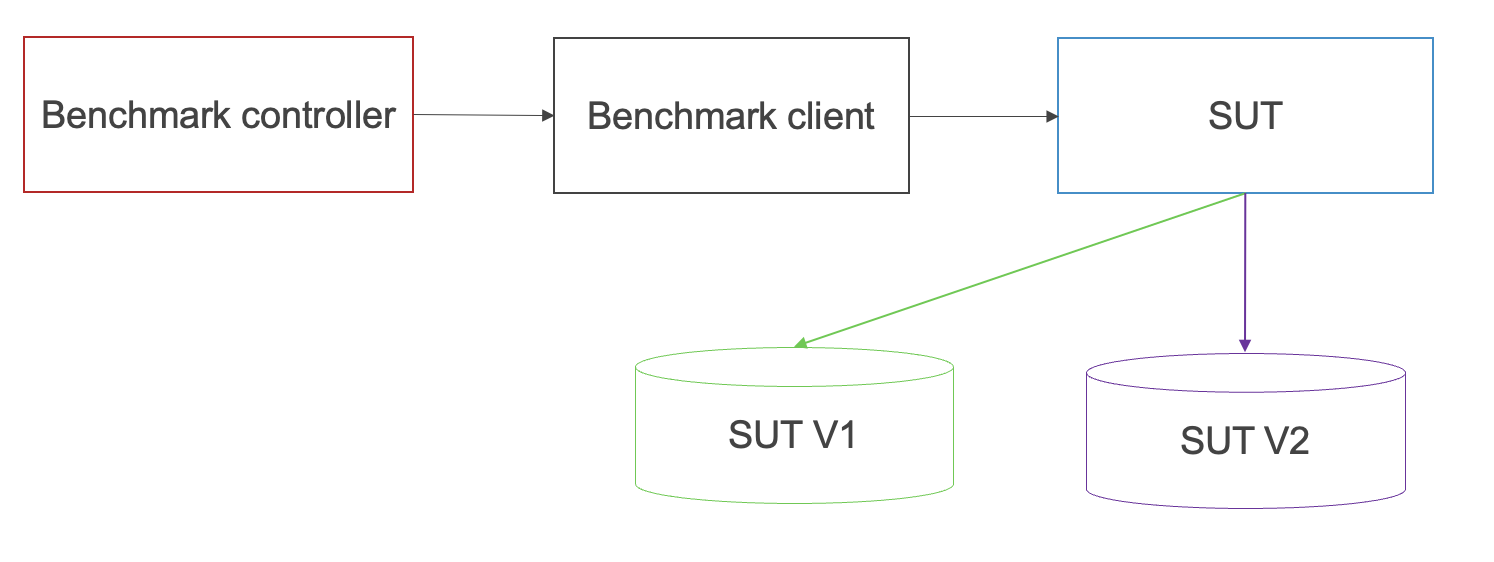
\includegraphics[width=\textwidth]{figures/Application setup.png}
        \caption{Application Benchmark Setup}
        \label{fig:applicationBenchmark-setup}
    \end{subfigure}
    \hfill
    \begin{subfigure}[b]{0.49\textwidth}
        \centering
        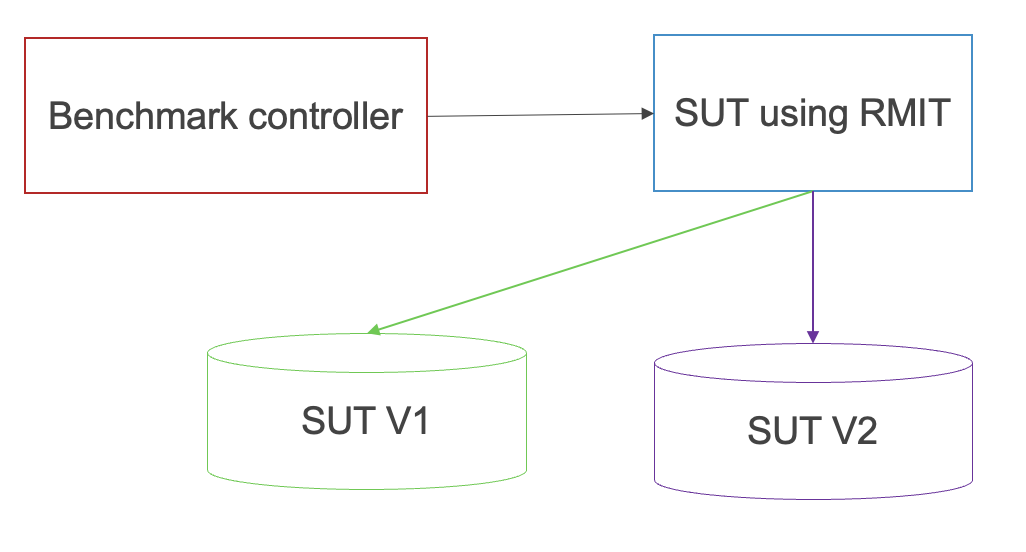
\includegraphics[width=\textwidth]{figures/Microbenchemark setup.png}
        \caption{Microbenchmark Setup}
        \label{fig:microbenchmark-setup}
    \end{subfigure}
    \caption{Benchmarks setup}
    \label{fig:benchmarks-setup}
\end{figure}

Additionally, we create another instance called a controller in both setups. The controller instance orchestrates the experiments with a startup script that will parallel start the application benchmark and the microbenchmarks. Since the experiments are done in parallel, the controller will start the application benchmark and the microbenchmarks in different terminal processes. Having the controller is helpful to avoid having control over the experiments on the local computer; since the experiments take a long time to complete, one will likely close the computer, restart, or close the terminal without the experiments finishing, thus losing the data collected. Therefore, having this approach prevents local machine disruptions that could lead to data loss or invalid results if the experiments were run locally. \\
Once the setup is complete and we created all the instances, the second phase starts, the installation phase. In this phase, we install the required software into the instances on each virtual machine. Key installations include GO, Docker, Git, benchmarking tools like VictoriaMetrics and GoAPIBenchmarkingScore (\ac{GoAbs}), and a Time series benchmark suite (\ac{TSBS}). All the virtual machines in both the microbenchmark and application benchmark are set up to run Debian-11 as the operating system and are deployed to the zone euro-west1-b. After we install the required tooling, we run another Ansible command to configure the \ac{SUT} for both the application benchmark and the microbenchmark.  \\
Lastly, the third phase is running the experiments. This phase comes into place once the installation is done. In this stage, the controller instance will be restarted, and the startup script will be triggered to execute the application benchmark and the microbenchmarks using benchmarking techniques, such as duet benchmarking for application benchmarks and Randomised Multiple Interleaved Trials (\ac{RMIT}) for microbenchmarks, to reduce external noise and improve data reliability. \\
After running the benchmarks, we collect the data from the experiments and analyze the results, which will be used to train and validate a ridge regression model. 


\subsection{Application benchmarks}
For the application benchmark, this research uses an open-source tool called the Time Series benchmark suite, further referred to as \ac{TSBS}. This tool was created to measure the performance of different Time Series databases, giving the developer a chance to compare them; one of those is VictoriaMetrics, which makes it easier to deploy the experiments to test the research question. \ac{TSBS} comes with predefined useCases to generate the workload for the \ac{SUT}s; depending on the useCase selected, one can get different workload data; one of the available useCases in \ac{TSBS} for VictoriaMetrics is the useCase "DevOps", which aligns perfectly with this research, as the main objective of this research is to allow developers to detect performance regressions faster. \\
As previously stated, application benchmarks deploy a \ac{SUT} to a real environment to detect performance changes. Therefore, to mimic a realistic setup, we set virtual machines (\ac{VM}s) from scratch for the application benchmarks and created 2 \ac{VM}s. The first runs the \ac{SUT},  and the second is a client in charge of generating and inserting the artificial loads into the \ac{SUT}. The reason behind this is to prevent the resources of the \ac{SUT} from being affected by the generation of artificial loads and their insertion in the \ac{SUT}. Thus, by separating this into two \ac{VM}s, we can guarantee that the \ac{SUT} only has the application load that will be tested. For the application benchmarks’ configuration, we use Docker to pull the image for each version configured in the configuration file and run the two Docker containers. \cref{tab:vm_configurations} shows the resources used for the virtual machines' configuration. \\
\begin{table}[ht]
    \centering
    \begin{tabular}{lccc}
        \toprule
        \textbf{Resource} & \textbf{Controller} & \textbf{Client} & \textbf{System Under Test (SUT)} \\
        \midrule
        Machine Setup & e2-medium & e2-standard-8 & e2-standard-4 \\
        Virtual CPUs & 2 & 8 & 4 \\
        Memory (GB) & 4 & 32 & 16 \\
        Disk Size (GB) & 50 & 50 & 50 \\
        \bottomrule
    \end{tabular}
    \caption{Virtual machine configurations for application benchmark}
    \label{tab:vm_configurations}
\end{table}
We use the e2-standard-4 virtual machine configuration, which allows us to divide four virtual \ac{CPU}s and 16 GB of memory into two Docker containers. Docker helped us limit the allowed CPU resources for the application benchmark, resulting in each container having 1.5 virtual \ac{CPU}s and 6 GB of memory available. This setup guarantees that the system under test is maxed out with artificial workloads and provides reliable results, ensuring that the system is under stress to be able to see and analyze its limits and detect performance changes. At the same time, we also have to guarantee that the client is not using over \text{60\%} of the resources to ensure that the client is not a bottleneck in this experiment. we changed the default disk size to 50 GB. With this setup in the application benchmark, we take advantage of the Duet benchmarking technique. We run the two versions of Victoria metrics in the same virtual machine using Docker to limit the resources available to each container. Hence, they have the same \ac{CPU} and \ac{RAM} to reduce external noise in the data generated by the application benchmark, ensuring that both versions of the \ac{SUT} operate under identical conditions. \\
\begin{table}[ht]
    \centering
    \begin{tabular}{l r}
        \toprule
        \midrule
        Number of Simulated Servers & 800 \\
        Sending Interval & 60s \\
        Simulated Duration & 120h \\
        Batch Size & 75 \\
        Number of Group-By Queries & 8,640 \\
        Number of Workers & 10 \\
        \bottomrule
    \end{tabular}
    \caption{Application benchmark parameters}
    \label{tab:applicationBenchmarkParameters}
\end{table}
This research executes the application benchmark in two steps. First, the benchmarking client generates data, which stresses the \ac{SUT}. Then, running the \ac{TSBS} workload using the DevOps use case generates data, as shown in \cref{tab:applicationBenchmarkParameters}, generates the data over five days with an interval of 60 seconds and uses the same interval to generate the queries that will be executed against the \ac{SUT}. Once the benchmark client generates the data for the 8640 queries, the next step is to insert the data into the \ac{SUT}. We run two terminal processes to insert the data into each Victoria metrics version. Next, we will wait for the data to be inserted into the two versions and give the \ac{SUT} 60 seconds to stabilize. \\
After this, we again create two new processes that will run the Group-by queries against each version of Victoria metrics, which conclude the execution of the application benchmark. Each experiment is repeated 10 times on the same pair of versions, e.g., v1.104- v1.105, another 10 times for v1.105-v1.106, 10 times for v1.106-v1.107, 10 times for v1.107- v1.108, and 10 times for v1.108-v1.109. We process the output files for each version and export the results to calculate the average load latency and the average Group-by query execution latency. We sum those values, resulting in the application benchmark’s average latency, and then compare them in the following section with the microbenchmark’s results to train and validate a ridge regression model. 

\subsection{Microbenchmarks}
On the other hand, to run the microbenchmarks, we use the Go API Benchmarking Score, also known as \ac{GoAbs}. This tool lets us execute microbenchmarks multiple times, having multiple iterations in each microbenchmark. The microbenchmarks were also executed into two versions, similar to the application benchmarks, to have more reliable results. \ac{GoAbs} allows us to enter a configuration file where one can define which functions of the microbenchmarks will be executed and how many times each function needs to be run. Additionally, one can determine how often we want the complete microbenchmark suite executed. Determining the execution time helps us obtain more data, giving us more reliable results. Furthermore, Grambow et al. \cite{grambow} adapted ABS by making some changes in the code and allowing two projects to be compared; the code changes consisted of only considering the common microbenchmarks in both versions to avoid analyzing irrelevant microbenchmarks and reducing costs and waste of resources. \\
For the microbenchmark setup, we only need to ensure that we have correctly installed GO so that the tool \ac{GoAbs} can be run correctly. In this case, as shown in \cref{tab:vm_configurations_micro}, we used the e2-standard-2 Virtual machine configuration, which provides two virtual \ac{CPU}s and 8 GB of memory. \\
This research follows the methodology proposed by Grambow et al. \cite{grambow} to execute the microbenchmarks. We will run the benchmark suite 3 times and each microbenchmark 5 times per run, giving us 45 measurements per microbenchmark. Considering that as Grambow et al. \cite{grambow}, this research executes two versions, obtaining a result of 45 measurements per microbenchmark per version. \\
Similar to the application benchmark, the microbenchmarks for the two versions are executed on the same virtual machine. The process for the microbenchmarks is much simpler; we clone the two different versions defined in the configuration file and execute \ac{GoAbs}to start running them. Lastly, to obtain accurate results, we use \ac{RMIT} which allows us to compare two microbenchmark versions fairly to avoid bias and reduce the probability of having the same results
\cite{japke2023earlymicrobenchmarkcatches}. \\
\begin{table}[ht]
    \centering
    \begin{tabular}{lccc}
        \toprule
        \textbf{Resource} & \textbf{System Under Test (SUT)} \\
        \midrule
        Machine Setup & e2-standard-2 \\
        Virtual CPUs & 2\\
        Memory (GB) & 8  \\
        Disk Size (GB) & 50 \\
        \bottomrule
    \end{tabular}
    \caption{Virtual machine configurations for microbenchmarks}
    \label{tab:vm_configurations_micro}
\end{table}

\subsection{Model Selection}
Performance prediction models help developers anticipate how software changes will affect system performance. To predict the application benchmark performance based on the microbenchmarks, we employed a multivariate linear regression model, more precisely, the ridge regression model. This model was selected because one of its primary properties is that it penalizes feature collinearity by incorporating a regularization strategy to remove it \cite{mcdonald2009ridgeregression}.  \\
Vrigazova \cite{vrigazova2021proportion} suggests splitting data into training and test data by allocating \text{80\%} for training and \text{20\%} for testing data. Therefore, this research will follow this suggestion after performing the data pre-cleanup. Then, we will fit the data into the model and apply the ridge regression. Once we obtain the quality metrics of the model, R-squared, and \ac{MSE}, we plan to load data that the model had never seen to test how accurate the predictions will be. As the \ac{SUT} obtains more releases, the likelihood of the microbenchmarks features changing is considerably high; therefore, we needed to make sure that the features that we trained to model with were present within any newly provided data in order to be able to use the model to predict the application benchmark. If we do not find the needed features, we will add 0 as the corresponding value, allowing the model to ignore this feature without compromising its predictions. 
\clearpage
\section{Evaluation}
Using the approach from \cref{cha:studydesign}, we now evaluate to what extent the microbenchmark results can predict a change in the application benchmark's results. We divide this section into two subsections. First, we describe the analysis to explain how the findings will be analyzed, and second, we outline the findings and implications of this study. 
\label{cha:evaluation}
\subsection{Analysis}
This research emphasizes two key areas of analysis to evaluate performance results of both application benchmark and microbenchmark and validate the proposed research question: (1) mean query rate and average execution time as performance metrics, and (2) R-squared and Mean Squared Error (\ac{MSE}) for model evaluation. Together, these sections provide a detailed understanding of how performance evolves across versions and how well the ridge regression model predicts application benchmark results using microbenchmark data.  \\
In order to follow best practices when performing both application and microbenchmarks, this research constantly measures the performance of the \ac{SUT} in pairs, where each benchmark compares two consecutive versions of the \ac{SUT} to capture incremental performance changes and reduce the probability of noise affecting the performance measurements. Therefore, each version was compared to its predecessor in all our experiments to evaluate performance changes over time. Specifically, as shown in \cref{tab:compared_versions}, we compared versions v1.104-v1.105, v1.105-v1.106, v1.106-v1.107, v1.107-v1.108 and v1.108-v1.109. This research considers this approach to maintain the reliability of performance comparisons across experiments. Thus, this approach allows us to assess performance shifts, leading to the identification of regressions or optimizations perceived across the compared pair of versions. \\
However, a challenge with this approach is that the bigger the difference between the pair of versions, the greater the chance that the number of common microbenchmarks will be reduced. This challenge is because future versions expect to include code changes that add and remove benchmarks that no longer apply to the newest release. For instance, it is not the same if we compare v1.104 with v1.107 because v1.104 may lack benchmarks that were added in v1.107, resulting in fewer comparable data points; hence, the number of common microbenchmarks between them is less than the common ones that the pair of versions of v1.106 and v1.107 have. Thus, comparing versions using the adjacent version provides us with more reliable and accurate results as it maintains a more significant amount of common microbenchmarks while minimizing noise and ensures that the performance difference can be attributed to the actual effect a code change has on the microbenchmark rather than environmental noise. 
\begin{table}[ht]
    \centering
    \begin{tabular}{c c c} % Bold headers
        \toprule
        \textbf{Version 1} & \textbf{Version 2} \\
        \midrule
        v1.104 & v1.105 \\
        v1.105 & v1.106 \\
        v1.106 & v1.107 \\
        v1.107 & v1.108 \\
        v1.108 & v1.109 \\
        \bottomrule
    \end{tabular}
    \caption{Pair of SUT versions compared}
    \label{tab:compared_versions}
\end{table}

\subsubsection{Performance metrics}
This research analyzes two performance metrics to measure the average time required to complete an operation. It calculates the mean query rate in the application benchmark and the average execution time for the microbenchmark. These performance metrics reflect how the system behaves and responds under load and how external conditions influence it by capturing overall performance trends, including occasional highs or lows. \\
This research aims to identify performance trends using the mean query rate and the average execution time of each pair of versions. Those values are passed to the ridge regression model to perform the prediction. Nevertheless, these metrics have a limitation, as they are calculated using averages; they are sensitive to outliers; thus, they must be considered correctly to avoid distorting performance measurements. However, ridge regression addresses this limitation by applying L2 regularization, which prevents the model from overfitting to outliers, smoothing the impact on high and low values, and allowing the model to learn general performance patterns while keeping away the external noise. Therefore, this regularization allows the model to consider both the mean and the outliers without overfitting the model. \\
The mean query rate and the average execution time metrics help us identify patterns to predict whether a new code version will lead to performance improvements or degradation. A decrease in these two metrics indicates optimization and faster execution times, whereas an increase may suggest performance regression.  

\subsubsection{R-Squared and MSE}
This research considers two main values, the R-squared and the mean square error (\ac{MSE}), to determine how well the ridge regression model performed \cite{mcdonald2009ridgeregression, chicco2021coefficientofdetermination, wang2009meansquareerror}. These metrics provide insights into the model’s ability to fit and predict data, helping assess prediction accuracy. The R-squared explains the proportion of the variance of the input features and performance seen in the model. Its value ranges between 0 and 1; the closer it gets to 1, the better the model fits \cite{chicco2021coefficientofdetermination}. In this analysis, a high R-squared value indicates that the model successfully captures the relationship between the versions changed and the performance output, indicating that the model successfully reflects performance trends influenced by code changes between versions. \\
However, the R-squared alone does not guarantee a good model performance; the \ac{MSE} must be considered. The \ac{MSE} calculates the average squared differences between predicted and actual values. Lower \ac{MSE} values are desirable, opposite to the R-squared. The lower the \ac{MSE}, the better the model, which indicates better prediction accuracy as it shows that the model’s predictions are closer to the actual values \cite{wang2009meansquareerror}. \\
Evaluating these two parameters together helps distinguish between overfitting and underfitting. It allows us to balance fit and generalization used in the training and test sets by explaining sufficient variance without incurring high prediction errors on unseen data by the model.  \\
Having a high R-squared and a low \ac{MSE} in the training set but a high \ac{MSE} in the test set makes the model overfitting. Overfitting means the model performs well during the training set but poorly in the testing set. \\
Overfitting suggests that the model memorizes training data instead of learning general trends. On the contrary, low R-squared and high \ac{MSE} on both the training and test sets make the model underfitting. Underfitting means the model performs poorly in training and test sets, suggesting it cannot capture the data complexity. \\
This research aims to portray a balanced ridge regression that is neither overfitting nor underfitting. The R-squared and \ac{MSE} values demonstrate that the model generalizes well across training and testing sets, indicating that it has learned performance patterns without relying on specific data. Making the model more robust to provide insightful performance predictions.


\subsection{Findings and Implications}
\label{cha:results}
This section presents the results obtained from the experiments and has the following subsections. First, we analyze the results obtained by the application benchmark, where we detect performance changes in the application environment. Second, we analyze the microbenchmark's results to determine how accurately the performance changes in microbenchmarks affect the performance prediction of the application benchmark suites. Finally, this research further analyzes the findings and implications, combining the application benchmarks and microbenchmark's results into the ridge regression model and how well the model performed before analyzing the individual results of both the application and microbenchmark. This research needs to verify that two things are successfully achieved to ensure accurate and reliable results: First, we must ensure that the \ac{SUT} is fully stressed before we analyze the results in both the application and microbenchmarks. 

\begin{figure}[!htbp]
    \captionsetup[subfigure]{list=true}
     \centering
     \begin{subfigure}[b]{0.7\textwidth}
         \centering
         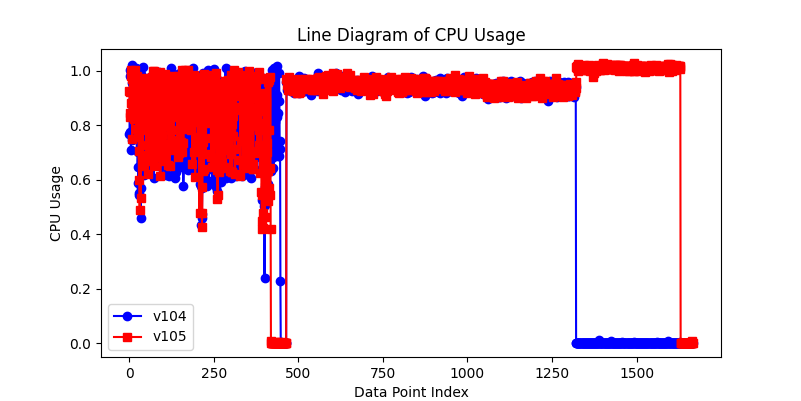
\includegraphics[width=\textwidth]{figures/applicationBenchmark_SUT.png}
         \caption{Application Benchmark}
         \label{fig:applicationBenchmark_SUT}
     \end{subfigure}
     \hfill
     \begin{subfigure}[b]{0.7\textwidth}
         \centering
         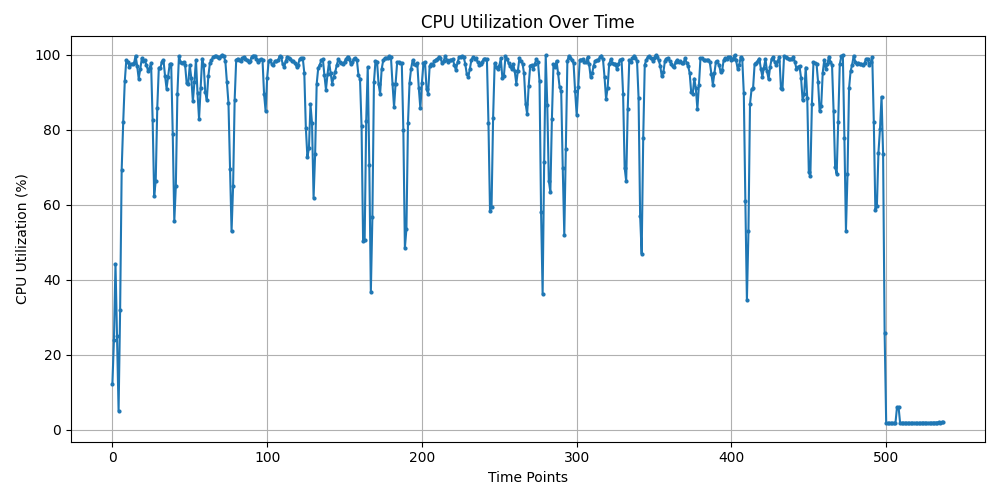
\includegraphics[width=\textwidth]{figures/cpu_utilization_analysis.png}
         \caption{Microbenchmark}
         \label{fig:microbenchmark_SUT}
     \end{subfigure}
     \caption{SUT under stress}
     \label{fig:SUT_under_streess}
\end{figure}

\cref{fig:SUT_under_streess} shows the \ac{SUT} of the application benchmark and the microbenchmark. Both show the \ac{SUT} as fully stressed. Second, we must verify that the application logs were completed successfully without errors. Ensuring this guarantees that the data was loaded successfully and that all the queries were run. 

\subsubsection{Application benchmark}
The application benchmark experiments required approximately 1.5 hours per run, split into two main phases: data insertion and Group-by query execution. The first phase is loading the 581.760.000 metrics into the  \ac{SUT}; this phase takes around 45 minutes to complete. The second phase executes the 8640 Group-By queries shown in \cref{tab:applicationBenchmarkParameters} in the system; it takes around 45 minutes to complete. This experiment successfully executes 50 application benchmarks, each pair of versions having 10 experiment runs. For application benchmarks, we compare the same pair of versions mentioned before in \cref{tab:compared_versions}: v1.104-v1.105, v1.105-v1.106, v1.106-v1.107, v1.107-v1.108, and v1.108-v1.109. \\
As application benchmarks have two phases, we have two metrics, one per phase. First, we have the mean insertion time for inserting the data into the \ac{SUT}, which refers to the first phase. Second, we have the mean query rate for executing all the Group-By queries in the second phase. The mean insertion time explains how much time, on average, each version of the application benchmark requires to insert 581.760.000 metrics, 51.840.000 rows, and 691.200 queries into the \ac{SUT}. \cref{fig:mean_inserts_time_all_runs-v104-v105,fig:mean_inserts_time_all_runs-v105-v106,fig:mean_inserts_time_all_runs-v106-v107,fig:mean_inserts_time_all_runs-v107-v108,fig:mean_inserts_time_all_runs-v108-v109} illustrate the variance in the mean insertion time during the data insertion phase across the 10 runs for each pair of versions v1.104-v1.105, v1.105-v1.106, v1.106-v1.107, v1.107-v1.108, and v1.108-v1.109, respectively.

\begin{figure}[ht]
    \captionsetup[subfigure]{list=true}
    \centering
    % -- Row 1: two subfigures --
    \begin{subfigure}[b]{0.48\textwidth}
        \centering
        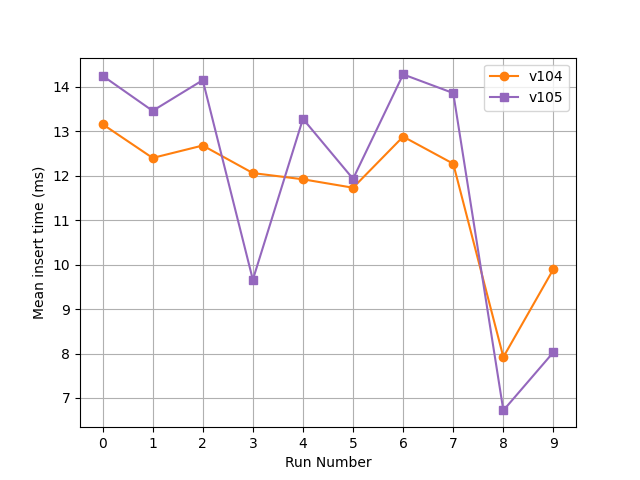
\includegraphics[width=\textwidth]{figures/mean_inserts_time_all_runs-v104-v105.png}
        \caption{v1.104--v1.105}
        \label{fig:mean_inserts_time_all_runs-v104-v105}
    \end{subfigure}
    \hfill
    \begin{subfigure}[b]{0.48\textwidth}
        \centering
        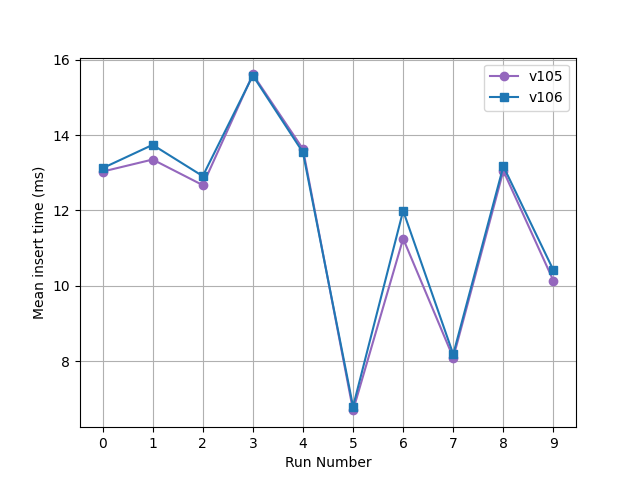
\includegraphics[width=\textwidth]{figures/mean_inserts_time_all_runs-v105-v106.png}
        \caption{v1.105--v1.106}
        \label{fig:mean_inserts_time_all_runs-v105-v106}
    \end{subfigure}

    \vskip\baselineskip  % vertical space between rows

    % -- Row 2: two subfigures --
    \begin{subfigure}[b]{0.48\textwidth}
        \centering
        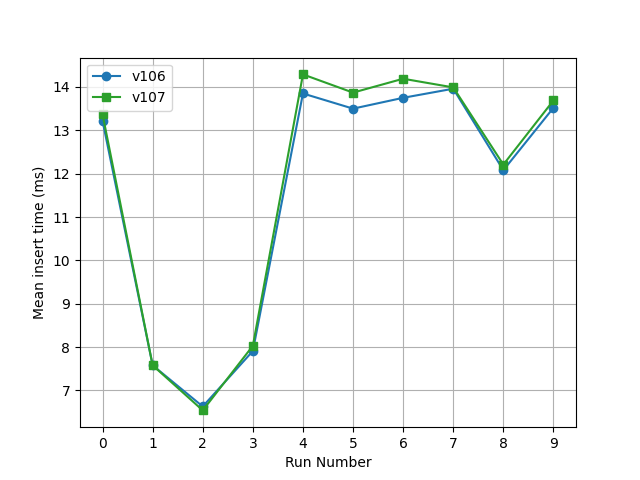
\includegraphics[width=\textwidth]{figures/mean_inserts_time_all_runs-v106-v107.png}
        \caption{v1.106--v1.107}
        \label{fig:mean_inserts_time_all_runs-v106-v107}
    \end{subfigure}
    \hfill
    \begin{subfigure}[b]{0.48\textwidth}
        \centering
        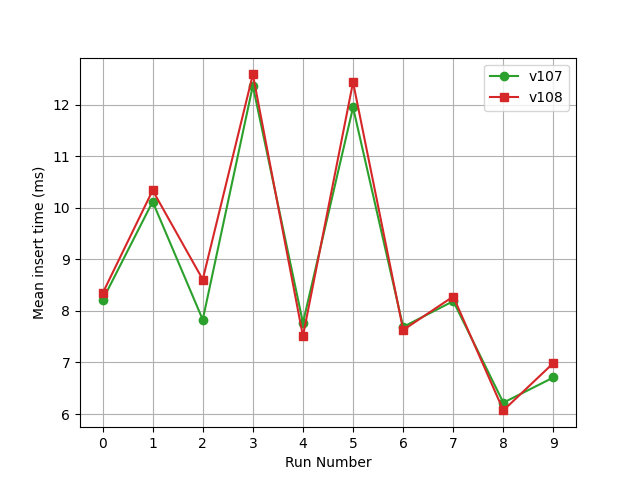
\includegraphics[width=\textwidth]{figures/mean_inserts_time_all_runs-v107-v108.png}
        \caption{v1.107--v1.108}
        \label{fig:mean_inserts_time_all_runs-v107-v108}
    \end{subfigure}

    \vskip\baselineskip  % vertical space between rows

    % -- Row 3: single subfigure --
    \begin{subfigure}[b]{0.48\textwidth}
        \centering
        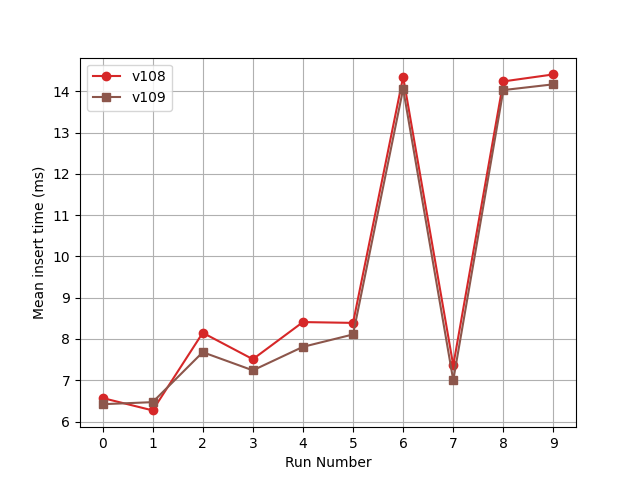
\includegraphics[width=\textwidth]{figures/mean_inserts_time_all_runs-v108-v109.png}
        \caption{v1.108--v1.109}
        \label{fig:mean_inserts_time_all_runs-v108-v109}
    \end{subfigure}

    \caption{Insert time}
    \label{fig:insertTime}
\end{figure}



\begin{figure}[ht]
    \captionsetup[subfigure]{list=true}
    \centering
    % -- Row 1: two subfigures --
    \begin{subfigure}[b]{0.48\textwidth}
        \centering
        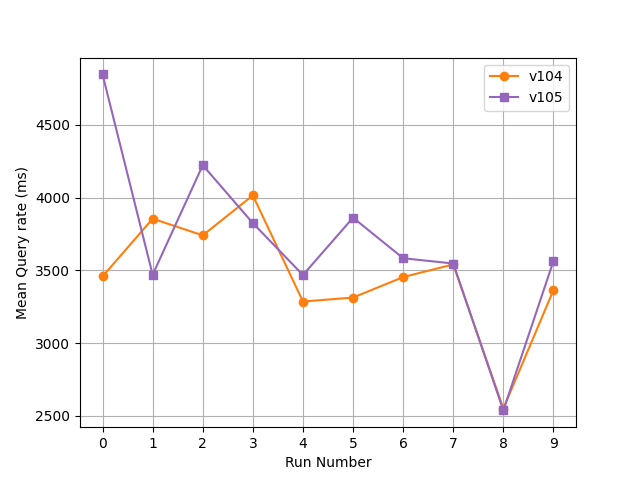
\includegraphics[width=\textwidth]{figures/mean_query_rate_all_runs-v104-v105.png}
        \caption{v1.104--v1.105}
        \label{fig:mean_query_rate_all_runs-v104-v105}
    \end{subfigure}
    \hfill
    \begin{subfigure}[b]{0.48\textwidth}
        \centering
        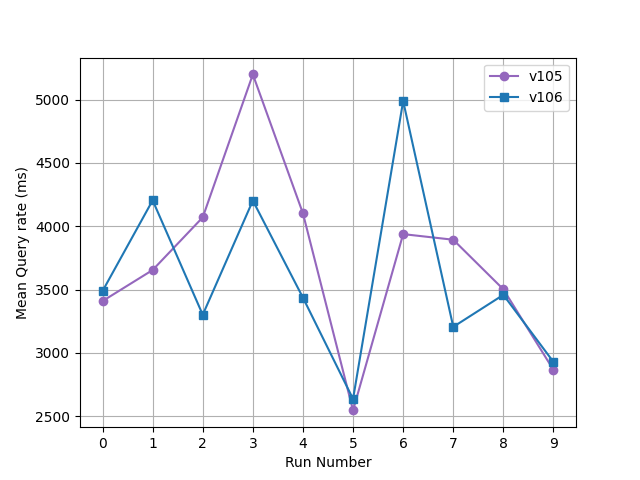
\includegraphics[width=\textwidth]{figures/mean_query_rate_all_runs-v105-v106.png}
        \caption{v1.105--v1.106}
        \label{fig:mean_query_rate_all_runs-v105-v106}
    \end{subfigure}

    \vskip\baselineskip  % vertical space between rows

    % -- Row 2: two subfigures --
    \begin{subfigure}[b]{0.48\textwidth}
        \centering
        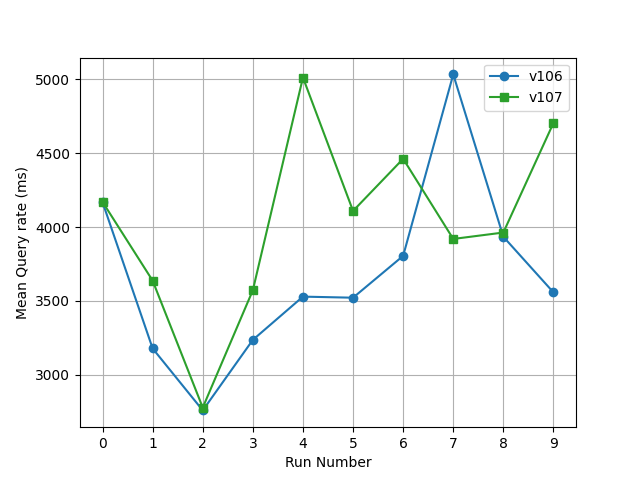
\includegraphics[width=\textwidth]{figures/mean_query_rate_all_runs-v106-v107.png}
        \caption{v1.106--v1.107}
        \label{fig:mean_query_rate_all_runs-v106-v107}
    \end{subfigure}
    \hfill
    \begin{subfigure}[b]{0.48\textwidth}
        \centering
        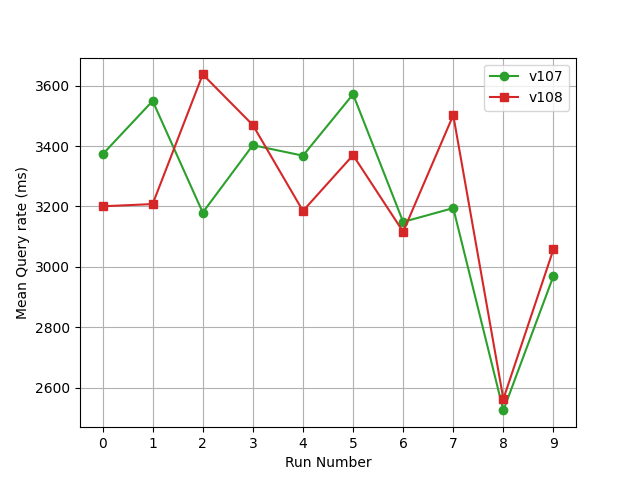
\includegraphics[width=\textwidth]{figures/mean_query_rate_all_runs-v107-v108.png}
        \caption{v1.107--v1.108}
        \label{fig:mean_query_rate_all_runs-v107-v108}
    \end{subfigure}

    \vskip\baselineskip  % vertical space between rows

    % -- Row 3: single subfigure --
    \begin{subfigure}[b]{0.48\textwidth}
        \centering
        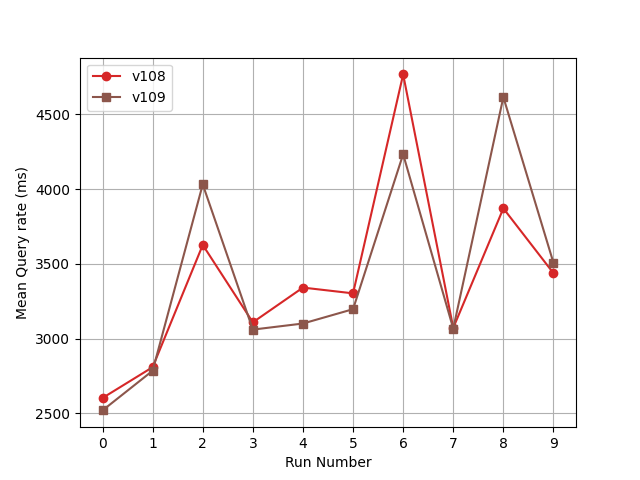
\includegraphics[width=\textwidth]{figures/mean_query_rate_all_runs-v108-v109.png}
        \caption{v1.108--v1.109}
        \label{fig:mean_query_rate_all_runs-v108-v109}
    \end{subfigure}

    \caption{Mean query rate for various version intervals.}
    \label{fig:mean_query_rate}
\end{figure}

\cref{fig:mean_inserts_time_all_runs-v104-v105,fig:mean_inserts_time_all_runs-v106-v107,fig:mean_inserts_time_all_runs-v105-v106,fig:mean_inserts_time_all_runs-v107-v108,fig:mean_inserts_time_all_runs-v108-v109}, show that the performance of each pair of versions is stable, ranging from 6 \ac{ms} to a maximum of 16 \ac{ms}. \cref{fig:mean_inserts_time_all_runs-v104-v105} portrays the biggest variation in the mean insert values between both versions. Meanwhile, \cref{fig:mean_inserts_time_all_runs-v105-v106,fig:mean_inserts_time_all_runs-v106-v107,fig:mean_inserts_time_all_runs-v107-v108,fig:mean_inserts_time_all_runs-v108-v109} show that both versions in each pair follow the same trend and have less variance between them.\\
Furthermore, the mean query rate of executing all the Group-By queries explains how much time, on average, each version of the application benchmarks requires to execute the 8640 group-by queries successfully.  \cref{fig:mean_query_rate} shows the variance of the mean query rate of executing all the Group-By queries over the 10 runs of the pair versions v1.104-v1.105, v1.105-v1.106, v1.106-v1.107, v1.107-v1.108 and v1.108-v1.109.  \\
As seen in  \cref{fig:mean_query_rate_all_runs-v104-v105,fig:mean_query_rate_all_runs-v105-v106,fig:mean_query_rate_all_runs-v106-v107,fig:mean_query_rate_all_runs-v107-v108,fig:mean_query_rate_all_runs-v108-v109},  the variance of the mean query rate of the pair versions was consistent, ranging from 2500 \ac{ms} to 5000 \ac{ms}. \cref{fig:mean_query_rate_all_runs-v107-v108} shows that the pair of versions with less variance was v1.107-v1.108, where the maximum value was 3600 \ac{ms} and the minimum 2500 \ac{ms}, matching the expectation that the newer the version is, the better the performance would be. The variance analysis across both phases helps us determine the consistency and reliability of each version's performance under load. Thus, the following section considers the mean latencies of both phases (data insertion and Group-by queries execution) as the dependent variable in the ridge regression model, as this is the value that the model proposed in this research aims to predict. 

\subsubsection{Microbenchmark}
After running the complete microbenchmark suite, we noticed that each microbenchmark run took around 8 hours to complete due to the setup configuration. \cref{tab:compared_versions} shows this research tested five pairs of versions: v1.104-v1.105, v1.105-v1.106, v1.106-v1.107, v1.107- v1.108 and v1.108-v1.109. Both pairs of versions, v1.104-v1.105 and v1.105-v1.106, were executed with 552 microbenchmarks, and versions v1.106-v1.107 and v1.107-v1.108 executed a total of 549 microbenchmarks, whereas version v1.108-v1.109 executed a total of 546 microbenchmarks. Confirming the assumption that as the software evolves over multiple versions, the greater the distance between one version and the other, the fewer common features will be present in both microbenchmarks’ versions. \\
Additionally, we noticed that the results do not contain a mean metric for the 10 runs executed; we had to perform a step where we got all the data from the different runs of the experiments to calculate the mean execution time metric by ourselves. In this step, we used Python to perform all the data transformations, specifically using libraries like numpy and Pandas. As a result, we calculated the mean for the three runs and five iterations, which gave 45 measurements for each of the microbenchmarks executed on each version. We sum this value with the other nine executions and divide by the number of runs (10), and that is how we calculate the mean of the microbenchmarks that help us clean up the model's data.  \\
Then, we proceeded to perform a collinearity analysis to improve the feature selection for the model, which allowed us to optimize the set of microbenchmarks provided to the model by eliminating the high collinearity between the microbenchmark's functions and removing redundant features. As a result, we will use a subset of microbenchmarks in the ridge regression model to make predictions of the application benchmark performance. \\
However, the model will be accurate and valuable only if it guarantees that the same subset of microbenchmarks will always be present in future versions. Otherwise, the non-present microbenchmarks will be replaced by 0 to avoid including invalid data that leads to wrong predictions. The mean execution time for each microbenchmark, calculated in \ac{ms}, provides insight into performance differences across versions. This metric helps us evaluate performance changes between the pair of versions in the  \ac{SUT}. \cref{tab:version_time} summarizes the mean execution time of each pair of versions. By comparing the mean execution time across versions, we can determine if its performance has improved or degraded. When comparing both versions, if the mean execution time increases, it may indicate a performance regression as it takes more time to execute the microbenchmark. On the contrary, if the mean execution time decreases, the performance improves, suggesting that the function is optimized, providing a faster execution time. Therefore, this comparison allows us to identify the performance impact that code changes have across the pair versions.  \\
\cref{tab:version_time} illustrates that the mean execution time in minutes between v1.104 and v1.105 is 488,489, the one for v1.105-v1.106 is 493,455, v1.106-v1.107 is 490,523, v1.107-v1.108 is 482,036, and v1.108-v1.109 is 484,105. These results show that the mean execution time between versions v1.104-v1.105 is lower than the pair of versions v1.105-v1.106 and v1.106-v1.107. On the other hand, the mean execution time between v1.107-v1.108 and v1.108-v1.109 is lower than the mean execution time of the pair version v1.104-v1.105. Therefore, \cref{tab:version_time} suggests that the performance in the pair version v1.104-v1.105 was better than the subsequent versions, meaning that v1.105-v1.106 and v1.106-v1.107 required more time to be successfully executed on average, which implies that the performance degraded in these two pair versions. Additionally, the performance of versions v1.107-v1.108 and v1.108-v1.109 improved, showing that they both required less time to complete than versions v1.104-v1.105. The increase and decrease in the mean execution time between these pair versions might be attributed to code changes or features implemented in the newer versions, affecting their performance. After performing the 10 runs for each pair of versions, each run will have the average execution time for each microbenchmark. The following section will use these results in our ridge regression model to help capture performance behavior and predict future performance trends.  

\begin{table}[ht]
    \centering
    
    \begin{tabular}{c c c} % Bold headers
        \toprule
        \textbf{Version} & \textbf{Minutes} & \textbf{Hours} \\
        \midrule
        v1.104 - v1.105 & 488.879 & 8.147 \\
        v1.105 - v1.106 & 493.455 & 8.224 \\
        v1.106 - v1.107 & 490.523 & 8.175 \\
        v1.107 - v1.108 & 482.036 & 8.033 \\
        v1.108 - v1.109 & 484.105 & 8.068 \\
        \bottomrule
    \end{tabular}
    \caption{Time Comparison Between Versions}
    \label{tab:version_time}
\end{table}


\subsubsection{Ridge regression Model}
Before we could use the data generated by the microbenchmarks and application benchmark in the ridge regression model, we noticed that the distribution of our data was not as linear as expected. Therefore, further analyses were conducted to improve the model's feature selection. We do an optimization that, in this case, was a pre-clean-up step for the data, where, with the help of a correlation matrix, we performed the feature selection step to determine how much the features were collinear with each other; this helped us reduce the number of microbenchmarks used as features in the model. \\
The ridge regression model uses the average execution time from the microbenchmarks as features and the mean query rate as the target variable. Then, the R-squared and \ac{MSE} metrics are calculated to indicate the model's accuracy.  \\
\cref{tab:threshold_metrics} shows the results of the threshold, features, R-squared, and \ac{MSE}. The threshold is the alpha parameter the ridge regression takes as an input to penalize the features to avoid overfitting the model. The features refer to the number of microbenchmarks used to train the model. R-squared and \ac{MSE} determine how good the model is.  \\
\cref{tab:threshold_metrics} that different thresholds were implemented with different amounts of features to analyze the changes in both R-squared and \ac{MSE}. However, due to the microbenchmarks' high collinearity, it was impossible to identify an alpha value that could explain how data was distributed, giving us a high R-squared and low \ac{MSE}. The results show that this model has a low R-squared and high \ac{MSE}, which means that the model presents overfitting. 

\begin{table}[ht]
    \centering
    \begin{tabular}{c c c c} % Bold headers
        \toprule
        \textbf{Threshold} & \textbf{Features} & \textbf{MSE} & \textbf{R²} \\
        \midrule
        0.0000100000 &  4   & 424344.5968 & -0.2093 \\
        0.0000010000 & 28   & 349287.0872 &  0.0046 \\
        0.0000001000 & 75   & 349287.0876 &  0.0046 \\
        0.0000000100 & 153  & 349286.7702 &  0.0046 \\
        0.0000000010 & 240  & 349300.2626 &  0.0046 \\
        \bottomrule
    \end{tabular}
    \caption{Performance Metrics at Different Thresholds}
    \label{tab:threshold_metrics}
\end{table}


\clearpage
\section{Discussion}
\label{cha:discussion}
This research aims to establish a predictive framework for application benchmark performance based on microbenchmark execution results. The study ensures that both benchmarking types are conducted in controlled yet realistic environments. The discussion below summarizes key insights acknowledges limitations and suggests further work that other researchers can do. 

\subsection{Application benchmarks and Microbenchmarks}
The application benchmark experiments, executed over five pairs of versions shown in  \cref{tab:compared_versions}—v1.104-v1.105, v1.105-v1.106, v1.106-v1.107, v1.107-v1.108, and v1.108-v1.109 revealed consistent performance trends under load. The two-phased approach, consisting of data insertion followed by query execution, provided a comprehensive view of the \ac{SUT}'s behavior and how it evolved between versions. \cref{fig:mean_inserts_time_all_runs-v104-v105,fig:mean_inserts_time_all_runs-v105-v106,fig:mean_inserts_time_all_runs-v106-v107,fig:mean_inserts_time_all_runs-v107-v108,fig:mean_inserts_time_all_runs-v108-v109,fig:mean_inserts_time_all_runs-v107-v108,fig:mean_query_rate_all_runs-v104-v105,fig:mean_query_rate_all_runs-v105-v106,fig:mean_query_rate_all_runs-v106-v107,fig:mean_query_rate_all_runs-v107-v108,fig:mean_query_rate_all_runs-v108-v109} clearly showed that, regardless of the model's limitations, performance changes across versions were evident in the graphs. \cref{fig:insertTime,fig:mean_query_rate} show that code changes lead to performance improvements or regressions, even when the current predictive model does not fully capture the underlying relationship and cannot adequately represent its link. \\
During the application benchmarks' execution, we identified several resource allocation challenges, particularly related to the \ac{SUT}'s we configured the virtual machines provisioned for the benchmark using the e2-standard-2 allocation of resources; however, during the data insertion phase, the \ac{SUT} encountered connection reset errors, which ended the insertion process and invalidated the run of the group-by queries. We no longer faced the error after increasing the memory and \ac{CPU} available to the docker containers while keeping the \ac{SUT} under heavy resource usage.\\
The adjustment required for memory and \ac{CPU} availability underlines an important distinction between application benchmarks and microbenchmarks. Since microbenchmarks measure the performance of specific functions, while application benchmarks measure the performance of the whole application, significantly more resources are required to simulate real-world workloads accurately. These additional resources, given to the application benchmark, led to a challenge when comparing performance measurements across benchmarking techniques as they created a difference in the setup of both benchmarks. However, as application benchmarks are supposed to require larger resource allocation than microbenchmarks to manage and provide realistic operating workloads, this research believes that this was expected and does not invalidate the results because application benchmarks operate in environments where resource constraints, I/O bottlenecks and concurrency effects impact performance. \\ 
On the other hand, even though microbenchmarks are easier to set up compared to application benchmarks as they focus solely on individual functions, this research finds that they took, on average, 8 hours to run, as shown in \cref{tab:version_time}. We expected the experiments to take longer due to the techniques applied when running the microbenchmarks. However, this will challenge including the microbenchmarks in \ac{CI}/\ac{CD} pipelines because, on the one hand, the microbenchmarks require enough repetitions to provide accurate results, and on the other hand, waiting 8 hours for the pipeline to finish is not feasible. Therefore, their applicability to broader system performance is limited despite being executed hundreds of times for reliability. Additionally, high collinearity and redundancy among several microbenchmarks make it difficult to directly link micro-level performance changes to application-level outcomes. Thus, a performance optimization that appears effective in a microbenchmark function may lead to different results in an application benchmark. Given these findings, further work must be done with essential care to manage resource allocation in future performance evaluations to maintain accuracy and ensure benchmarking outcomes remain valid and comparable across various test environments. \\
Another challenge faced when running the microbenchmarks was the tool \ac{GoAbs} used to measure the microbenchmarks. This research also presented issues with the tool used to run microbenchmarks because, as stated before, this tool was modified by Grambow et al. \cite{grambow} and there was no clear documentation on how to be able to compare a pair of \ac{SUT}. This research fully relies on the modification made and only evaluates correctly the microbenchmarks that are common to both pairs of versions that are being tested.

\subsection{Challenges in Predicting Performance with Ridge Regression}
We use ridge regression to predict application benchmark performance based on microbenchmark results. This research uses Ridge regression due to its ability to handle collinearity through L2 regularization, which reduces the impact of highly correlated features \cite{mcdonald2009ridgeregression}. This research used one of the most common methods to measure errors when performing regressions: the Mean Square Error (\ac{MSE}) \cite{wang2009meansquareerror} and R-squared \cite{chicco2021coefficientofdetermination} as main metrics to be able to determine if their model was performing well or poorly. Furthermore, to select the best set of features possible for the model, we performed a collinearity analysis between the features to reduce the complexity of the model and have better results. In order to perform this analysis, we attempt to use two known methods; the first one is Principal Component Analysis, further referred to as Principal Component Analysis \ac{PCA} \cite{Jolliffe2002PCA}, and the Variance Inflation Factor, further referred to as Variance Inflation Factor \ac{VIF} \cite{thompson2017extractingVIF}. Despite our efforts, none of the mentioned methods yielded good results for the model. We will start by analyzing the efforts taken to perform \ac{PCA}, and then we will move to analyze \ac{VIF}.  \\ 
Jolliffe \cite{Jolliffe2002PCA} states that \ac{PCA} selects components to explain the most variation possible from the original variables in the features of microbenchmarks. However, this does not guarantee that the selected components will be the best for regression prediction. More importantly, another known limitation of \ac{PCA} is that this method assumes a linear transformation of the data \cite{Jolliffe2002PCA}, which is not the case in our research, as shown in \cref{cha:evaluation}. These two limitations of \ac{PCA} and the collinearity of the features did not allow for a dimensional reduction to select the best features possible to use in ridge regression. Some options can be applied to overcome the limitations of \ac{PCA}. Schölkopf et al. \cite{scholkopf1998nonlinearcomponent} state that a Kernel \ac{PCA} can address nonlinear data by mapping the features into a higher-dimensional space and then applying \ac{PCA}. However, due to a lack of expertise in advanced dimensionality reduction techniques, this research did not attempt to address these limitations. \\
The second method we attempted to use was \ac{VIF}; after this research failed to use \ac{PCA} to perform the feature selection for the model, we moved to analyze the collinearity of the features. Although Ridge regression has an L2 regularization that penalizes the features for their collinearity, this regression method presents some limitations when features have high collinearity. Therefore, as suggested by Thompson et al. \cite{thompson2017extractingVIF}, to address the high collinearity between the features, we attempted to use \ac{VIF} to remove highly correlated features. However, given the distribution of the data seen in \cref{fig:distribution_BenchmarkMergeBlockStreamsFourSourcesWorstCase-2,fig:distribution_BenchmarkParseProtobufRequest_scopes_1_rows_100_attributes_5-2,fig:distribution_BenchmarkQueueThroughputConcurrent_block,fig:distribution_BenchmarkUnmarshalDeltaConstArray-2}, \ac{VIF} is too strict to be applied for feature selection, as after running \ac{VIF}, we notice that the number of features selected was zero. This makes sense because, as stated before, we discovered that the collinearity between the microbenchmarks is very high.  \\
Given the poor results obtained by \ac{PCA} and \ac{VIF}, we decided to do a collinearity matrix between the features and remove the ones that were above a threshold of \text{99\%}, ultimately giving us the best \ac{MSE} and R-squared metrics. \\
However, the low R-squared values and high (\ac{MSE}) results show that the model suffers from overfitting. Indicating that ridge regression struggled to generalize effectively, limiting its reliability in predicting real-world application performance using microbenchmark results. Lastly, as also shown in \cref{fig:distribution_BenchmarkMergeBlockStreamsFourSourcesWorstCase-2,fig:distribution_BenchmarkParseProtobufRequest_scopes_1_rows_100_attributes_5-2,fig:distribution_BenchmarkQueueThroughputConcurrent_block,fig:distribution_BenchmarkUnmarshalDeltaConstArray-2} some clusters of points seem to show a distribution that might be explained by a linear regression method; this research does not analyze the data further due to time limitations and lack of expertise on how to perform this adjustment.  \\
\begin{figure}[!htbp]
    \captionsetup[subfigure]{list=true}
    \centering
    % -- Row 1: two subfigures --
    \begin{subfigure}[b]{0.9\textwidth}
        \centering
        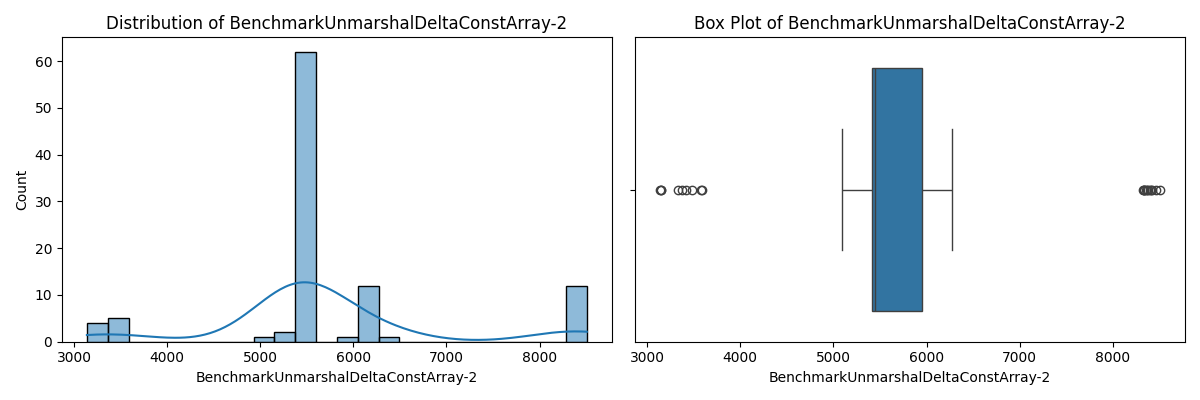
\includegraphics[width=\textwidth]{figures/distribution_BenchmarkUnmarshalDeltaConstArray-2.png}
        \caption{BenchmarkUnmarshalDeltaConstArray-2}
        \label{fig:distribution_BenchmarkUnmarshalDeltaConstArray-2}
    \end{subfigure}
      \vskip\baselineskip  % vertical space between rows
    \begin{subfigure}[b]{0.9\textwidth}
        \centering
        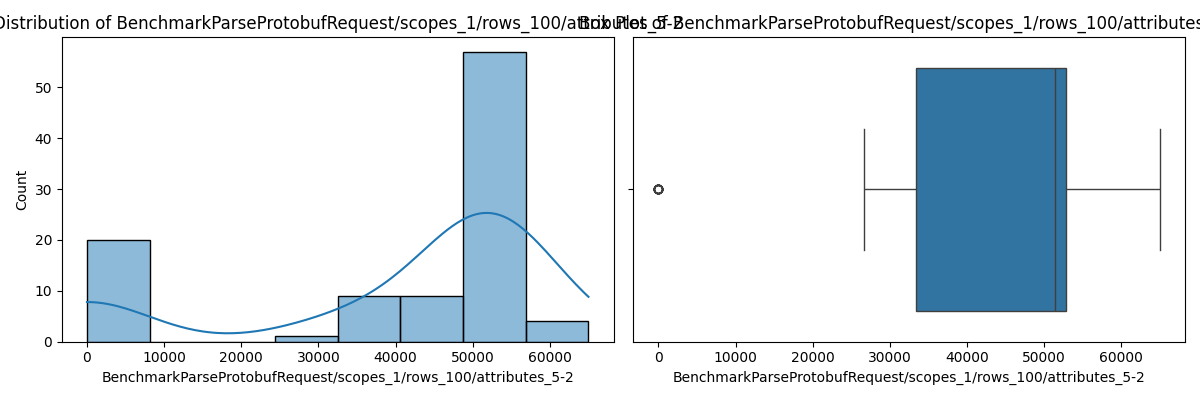
\includegraphics[width=\textwidth]{figures/distribution_BenchmarkParseProtobufRequest_scopes_1_rows_100_attributes_5-2.png}
        \caption{BenchmarkParseProtobufRequest-scopes-1-rows-100-attributes-5-2}
        \label{fig:distribution_BenchmarkParseProtobufRequest_scopes_1_rows_100_attributes_5-2}
    \end{subfigure}
          \vskip\baselineskip  % vertical space between rows
    \begin{subfigure}[b]{0.9\textwidth}
        \centering
        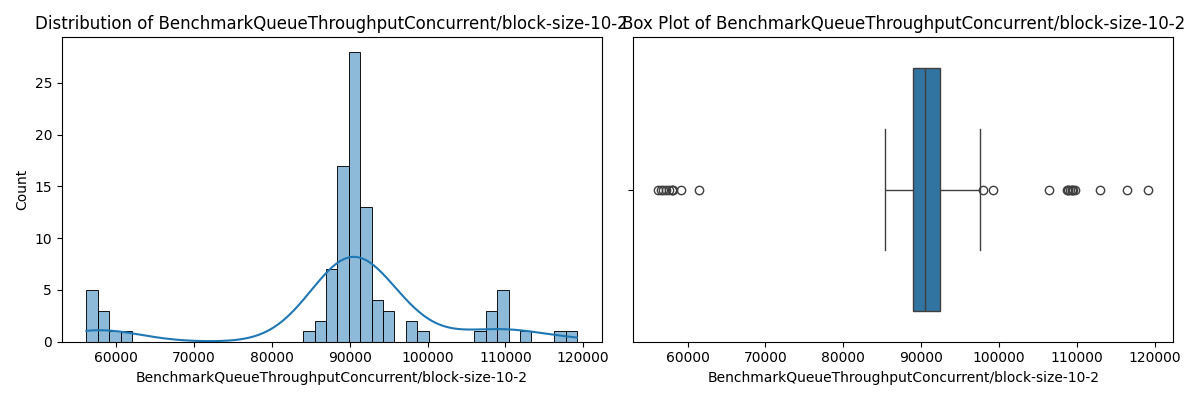
\includegraphics[width=\textwidth]{figures/distribution_BenchmarkQueueThroughputConcurrent_block-size-10-2.png}
        \caption{BenchmarkQueueThroughputConcurrent}
        \label{fig:distribution_BenchmarkQueueThroughputConcurrent_block}
    \end{subfigure}

    \vskip\baselineskip  % vertical space between rows
    \begin{subfigure}[b]{0.9\textwidth}
        \centering
        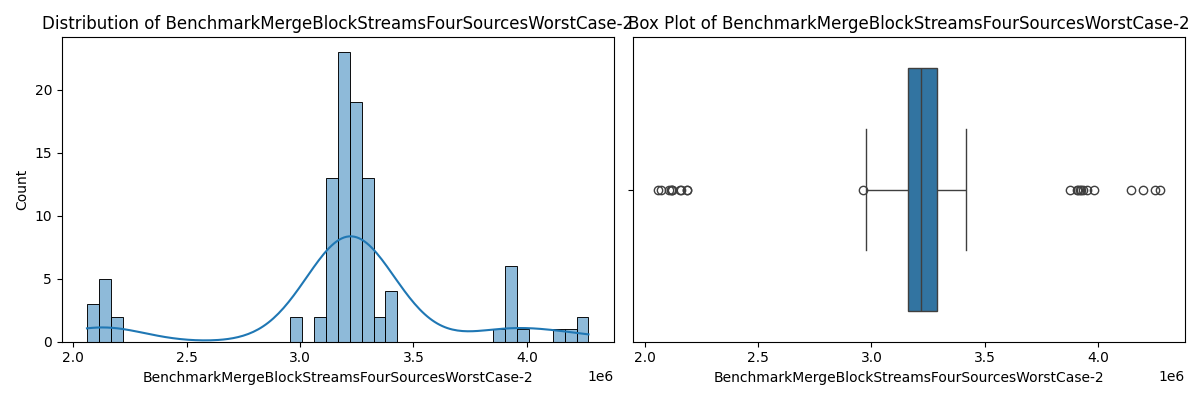
\includegraphics[width=\textwidth]{figures/distribution_BenchmarkMergeBlockStreamsFourSourcesWorstCase-2.png}
        \caption{BenchmarkMergeBlockStreamsFourSourcesWorstCase}
        \label{fig:distribution_BenchmarkMergeBlockStreamsFourSourcesWorstCase-2}
    \end{subfigure}
    \caption{Distribution Microbenchmarks}
    \label{fig:DistributionMicrobenchamrk}
\end{figure}
\cref{fig:distribution_BenchmarkUnmarshalDeltaConstArray-2,fig:distribution_BenchmarkParseProtobufRequest_scopes_1_rows_100_attributes_5-2,fig:distribution_BenchmarkMergeBlockStreamsFourSourcesWorstCase-2,fig:distribution_BenchmarkQueueThroughputConcurrent_block}
reveal distribution patterns that undermine our model. These do not follow a normal distribution presented across the benchmark functions. Instead, these figures present asymmetry, which prevents the ridge regression models from obtaining accurate results, instead presenting a high variance of the execution time leading to a fluctuating value across the experiment and a distribution where a significant number of observations have long tails toward higher execution times. These three key aspects explain why the ridge regression model fails to explain effectively and why alternative modeling techniques may be necessary to prove further the correlation between microbenchmarks and applications benchmarks performance.  

\begin{figure}[ht]
    \captionsetup[subfigure]{list=true}
    \centering
    \begin{subfigure}[b]{0.49\textwidth}
        \centering
        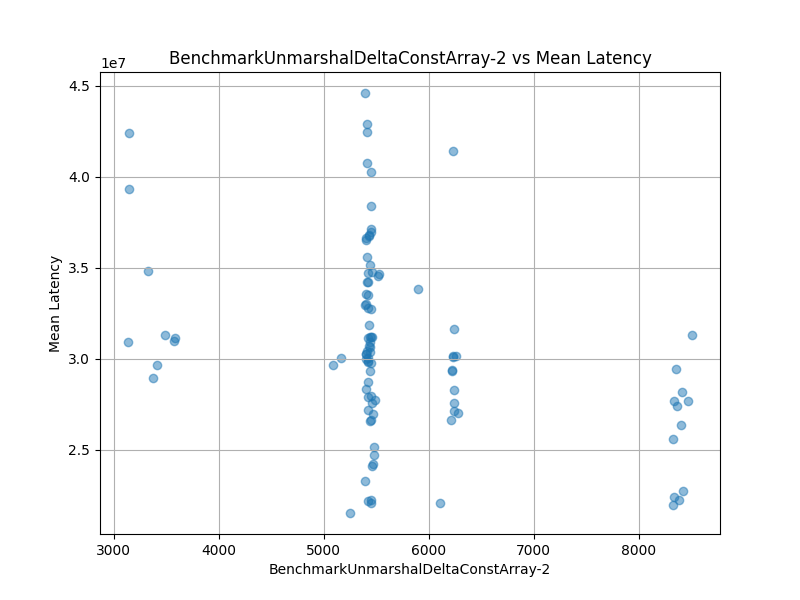
\includegraphics[width=\textwidth]{figures/BenchmarkUnmarshalDeltaConstArray-2_vs_mean_latency.png}
        \caption{BenchmarkUnmarshalDeltaConstArray vs mean query rate}
        \label{fig:BenchmarkUnmarshalDeltaConstArray-2_vs}
    \end{subfigure}
    \hfill
    \begin{subfigure}[b]{0.49\textwidth}
        \centering
        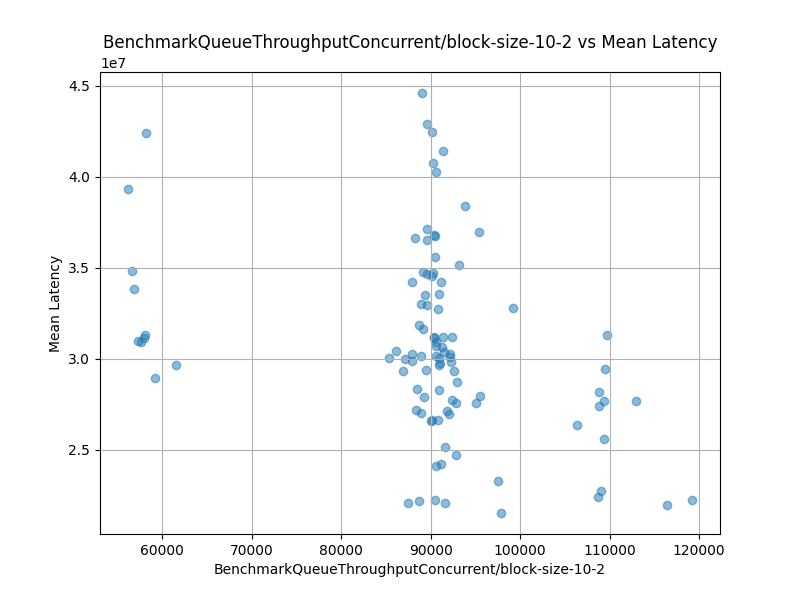
\includegraphics[width=\textwidth]{figures/BenchmarkQueueThroughputConcurrent_block-size-10-2_vs_mean_latency.png}
        \caption{BenchmarkQueueThroughputConcurrent vs mean query rate}
        \label{fig:BenchmarkQueueThroughputConcurrent_vs_mean_latency}
    \end{subfigure}

    \vskip\baselineskip  % vertical space between rows

    \begin{subfigure}[b]{0.45\textwidth}
        \centering
        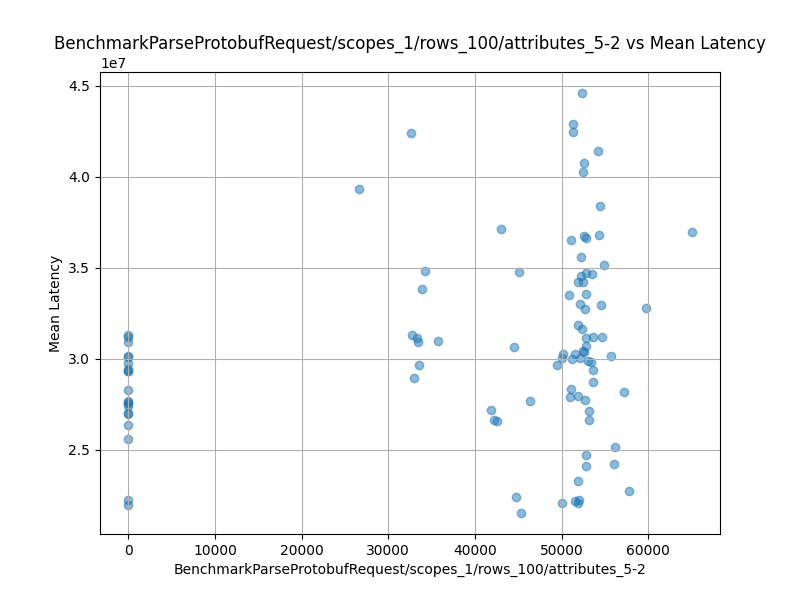
\includegraphics[width=\textwidth]{figures/BenchmarkParseProtobufRequest_scopes_1_rows_100_attributes_5-2_vs_mean_latency.png}
        \caption{BenchmarkParseProtobufRequest-scopes-1-rows-100-attributes-5-2 vs mean query rate}
        \label{fig:BenchmarkParseProtobufRequest_scopes_1_rows_100_attributes_5-2_vs_mean_latency}
    \end{subfigure}
    \hfill
     \begin{subfigure}[b]{0.45\textwidth}
        \centering
        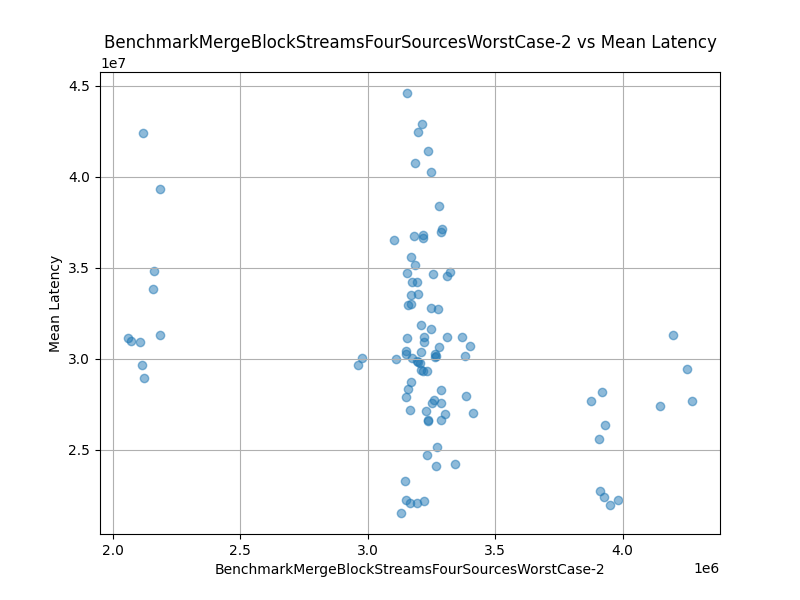
\includegraphics[width=\textwidth]{figures/BenchmarkMergeBlockStreamsFourSourcesWorstCase-2_vs_mean_latency.png}
        \caption{BenchmarkMergeBlockStreamsFourSourcesWorstCase vs mean query rate}
        \label{fig:BenchmarkMergeBlockStreamsFourSourcesWorstCase-2_vs_mean_latency}
    \end{subfigure}
    \caption{Microbenchmark vs mean rate query}
    \label{fig:micro-vs-mean-query}
\end{figure}

\cref{fig:BenchmarkQueueThroughputConcurrent_vs_mean_latency,fig:BenchmarkUnmarshalDeltaConstArray-2_vs,fig:BenchmarkParseProtobufRequest_scopes_1_rows_100_attributes_5-2_vs_mean_latency,fig:BenchmarkMergeBlockStreamsFourSourcesWorstCase-2_vs_mean_latency} confirm that the relationship between microbenchmark execution and application latency is not linear. We observe a vertical concentration of data points, indicating microbenchmark values do not correlate linearly with the mean query rate. \\
Instead, the mean query rate variates significantly for similar microbenchmark values, indicating that other factors influence performance changes beyond what our current model captures. These findings confirm that ridge regression, which assumes a linear relationship, is not well-suited for such variations, resulting in limited predictive accuracy. \\
\cref{fig:distribution_BenchmarkMergeBlockStreamsFourSourcesWorstCase-2}
portrays evidence that overfitting remains a core challenge and that increasing the number of pairs of versions does not resolve the model generalization problem. Instead, \cref{fig:DistributionMicrobenchamrk} suggests that the model memorizes behavioral patterns from the training but fails to apply them to the new data. Collinearity continues to challenge the models by adding noise to the predictions; hence, the model struggles to find an appropriate function to predict the application's performance based on microbenchmarks. \\
Even though Grambow et al. \cite{grambow} research showed that microbenchmark results could serve as a proxy for application benchmark performance (despite certain limitations), we could not replicate or refute his findings in our study, as our modeling approach did not yield robust predictions to confirm or contradict his results. These outcomes suggest that unless the effects of data distribution are carefully addressed, future research might expand on Grambow et al. \cite{grambow} research by applying more advanced statistical models or alternative regression techniques to evaluate whether microbenchmarks can reliably predict application-level performance.

\subsection{Limitations and Future Research}
\label{cha:limitationsFurtherWork}
This study provides valuable insights into comparing microbenchmark and application benchmarks. However, important limitations present in this research must be analyzed so that further research can use this work as a baseline to improve different aspects of the model’s feature selection and possibly get more accurate results. \\
When using statistical models to predict any value, the amount of data we have plays a significant role in how good the predictions might be; hence, one limitation in this study is the number of tested versions. This research conducted the experiments on a limited selection of pairs of versions, which may not fully reflect long-term performance trends or capture all possible variations across different software updates. It is probable that they do not accurately represent long-term performance trends.
Moreover, using an average-based performance metric is another limitation of this research; the detected outliers while running experiments highly influence average metrics results because they might introduce noise into the overall results, leading to inaccurate and poor performance conclusions. For this matter, future research should explore using other metrics that are not as sensitive to outliers, for instance, using median performance metrics; by implementing this metric type, further research could minimize the impact of unusual outliers in the overall performance result and obtain a more suitable model that proves a correlation between the performance change detected in a microbenchmark and its impact on the application’s benchmark performance.  \\
Additionally, the fact that this research evaluated only one system (VictoriaMetrics) is another limitation of this study. Even though relying on VictoriaMetrics allowed us to do an in-depth analysis by running the application benchmark and microbenchmark results on the same SUT, it limits the applicability of the findings to other SUTs because other optimizations might need to be done in different systems under tests which might influence the overall performance results of the application benchmark and microbenchmarks. \\
Lastly, this study uses a ridge regression model to predict if microbenchmark results predict the application benchmark performance. Even though ridge regression helps manage collinearity among features, its linear nature makes it less effective in capturing complex patterns in performance data. Therefore, we recommend that further research focus on more advanced methods to predict performance, such as decision trees or deep learning models, and see if we get reliable results. Thus, further research can use these results to investigate more about the clusters found in the distribution of the data shown in \cref{fig:distribution_BenchmarkMergeBlockStreamsFourSourcesWorstCase-2,fig:distribution_BenchmarkParseProtobufRequest_scopes_1_rows_100_attributes_5-2,fig:distribution_BenchmarkQueueThroughputConcurrent_block,fig:distribution_BenchmarkUnmarshalDeltaConstArray-2} and analyze if the clusters that present a better linear distribution would better fit a linear regression method. In addition to this, a dimensionality reduction could be applied to improve accuracy. Addressing these challenges would improve microbenchmark-based performance models' predictability and increase their ability to detect significant application benchmark performance trends. Future research can refine the benchmarking process to get more accurate results by incorporating more advanced modeling techniques, expanding dataset coverage, and validating results across multiple database systems, improving its value in assessing software performance under real-world conditions.  
\clearpage
\section{Related Work}
\label{cha:relatedWork}
A lot of research focuses on key areas when discussing benchmarking. This research considers the following related work areas to perform the experiments and analyze the results. We focus on two main sections: balancing accuracy and execution time and cloud benchmarking, as they provide the fundamental knowledge needed to perform the experiments. 

\subsection{Balancing accuracy and Execution Time}
In benchmarking, one of the challenges developers face is the tradeoff between costs and execution time \cite{japke2023earlymicrobenchmarkcatches, grambow, grambow2021usingApplication, alghamdi2023towards, laaber2021applyingtcp, he2019statistics, grambow2020benchmarkingMicroservicesperformance}. The longer developers execute the benchmark, the higher the costs; however, if the benchmark is not executed enough, it will lead to inaccurate results. Therefore, a balance is needed. Besides the approach used in this study, researchers use other approaches that focus on reducing the benchmark execution. Approaches like implementing test case prioritization \cite{laaber2021applyingtcp, laaber2019continuous, mostafa2017perfrankerprioritization, laaber2022multi}, stopping the benchmark when the conditions have high confidence of getting accurate results \cite{he2019statistics}, reducing redundancies by optimizing microbenchmarks \cite{grambow, grambow2021usingApplication, de2017perphecyperformance}, applying a principal component analysis \ac{PCA} \cite{trancoso2005reducingTPC} are commonly used when researching reduction of benchmarking execution times.\\
Laaber et al. \cite{laaber2021applyingtcp} explore using software microbenchmarks in performance testing pipelines using a test case prioritization \ac{TCP} approach. Demonstrating that coverage-based prioritization can be applied to microbenchmarks, allowing performance testers to schedule and run the most important benchmarks first. Laaber et al. \cite{laaber2021applyingtcp} use \ac{TCP} strategies in functional testing but adapt them to handle the continuous, distribution-based results common in performance evaluations. Notably, Laaber et al. \cite{laaber2021applyingtcp} found that prioritizing benchmarks by either their total coverage (how many project methods a benchmark touches) or additional coverage (the unique methods each benchmark tests beyond what has already been covered) can detect significant performance regressions earlier—thereby lowering the time needed to receive actionable feedback. The fewer microbenchmarks we run, the faster the suite will complete; therefore, the costs will be reduced. Thus, removing redundant tests and running only the most important tests saves time and costs while performing the benchmark suite without compromising the results. Therefore, This approach has the potential to streamline model training and improve performance estimates, ultimately providing faster, more precise feedback during the software development cycle.  \\
Japke et al. \cite{japke2023earlymicrobenchmarkcatches} created a \ac{SUT} using a microservice application testbed application, evaluating a flight booking service using application benchmarks and microbenchmarks. In their study, they conclude that although microbenchmarks detect performance issues much earlier than application benchmarks, application benchmarks continue to be more effective due to the cost and time associated with running the full suite of microbenchmarks.   \\
In our study, we ran the experiments using the full microbenchmark suite in a \ac{SUT} used in production environments. While performing our benchmarks, one of the biggest challenges was that the microbenchmark suite changed between versions; as expected, some microbenchmarks were no longer necessary and thus were removed from the code, while adding some new ones; this level of complexity was removed entirely by not using a \ac{SUT} deployed in production. This microbenchmark suite change was the most significant disadvantage of the results presented by Japke et al. \cite{japke2023earlymicrobenchmarkcatches}. Nevertheless, Japke et al. \cite{japke2023earlymicrobenchmarkcatches} implemented \ac{RMIT} duet benchmark techniques to reduce the noise from the cloud, giving robustness to their results. We also follow those techniques, deploying different versions of \ac{SUT} seen in \cref{tab:version_time} aand then running the application benchmark and microbenchmarks. Although we did not deploy the same version to run the benchmarks, the idea of using these techniques is to reduce the influence of cloud variability on the \ac{SUT}. So if version v1.104 was affected by any external factor, the assumption is that v1.105 will also be affected as they were deployed in the same Virtual machine. In our study, we experienced a similar behavior where the entire run of the microbenchmark suite took around 8 hours to complete. \\ 
In contrast, the application benchmark duration was considerably less, with an average time of one hour and thirty minutes. However, Japke et al. \cite{japke2023earlymicrobenchmarkcatches} contributions clearly show that microbenchmarks detect performance issues faster despite executing them longer. Although our model could not provide a good prediction, we also see that the microbenchmark data shows a performance improvement during the comparison of the different pairs, except in one version, where both application benchmark and microbenchmark present a downgrade in performance. This strengthens the purpose of attempting to predict application benchmarks using microbenchmarks, as our data also shows that microbenchmark performance varies similarly to application performance when testing different versions. Lastly, using techniques like the one mentioned earlier, \ac{TCP} by Laaber et al. \cite{laaber2021applyingtcp} we can considerably reduce the time it takes to run the microbenchmark suite, making it more efficient without compromising the data results.  \\
Grambow et al. \cite{grambow2021usingApplication} propose another approach to reduce the time of the microbenchmark execution and increase its relevance by mapping microbenchmark suites to application call graphs to determine if a system under test covers with microbenchmarks the functions used by the application benchmark. Firstly, they run an application benchmark as a base and record the call graphs to capture which functions have been used; then, they compare the result of the call graph to the microbenchmark suite to determine the coverage from microbenchmarks of the functions the application benchmark has used. This approach not only improves the time execution time and the relevance of the microbenchmarks but also serves as a guide to the developers to identify which portions of the code have yet been tested and should be covered; therefore, it serves as a starting point on how to improve the reliability of the \ac{SUT}, although having the microbenchmark test cover the complete \ac{SUT}, it does not guarantee detection of performance issues. Nonetheless, having good test coverage for your system is always a good practice. One challenge in our research was that the microbenchmark suite was too big; with \ac{TCP}, we knew that not all microbenchmarks are equally important as there are sometimes redundancies between the microbenchmarks. Grambow et al. \cite{grambow2021usingApplication} fits perfectly as a pre-step execution where one can filter the microbenchmarks used by the application benchmark and, therefore, have a smaller subset as features, reducing the model complexity. In another research, Grambow et al. \cite{grambow} investigated further if an optimized microbenchmark suite detects the same performance changes as an application benchmark; they analyze two-time series databases where first they apply the technique about call graphs mentioned before to optimize the microbenchmark suite and then compare the results with the application benchmark, with this approach they conclude that there was not a clear benefit of using an optimized version of the microbenchmark suite as a proxy. However, it serves as alternative performance feedback for developers in specific situations. In our study, we can also confirm that for the ridge regression, it did not matter how many microbenchmarks were selected as features; it always yielded an inferior R-squared result, but we do not think these results are directly related to the number of microbenchmarks selected but instead with the similarity from the microbenchmarks, if further research address this topic, then the using leveraging the research by Grambow et al. \cite{grambow} we could have a model that at performs better when explaining the distribution of the data. \\
Trancoso et al. \cite{trancoso2005reducingTPC} propose yet another approach to reduce the time it takes to execute the benchmarks and argue that microbenchmarks are not able to capture the full details of an application; they select a subset of queries using a statistical method, principal component analysis \ac{PCA} to reduce the number of queries that are necessary to obtain an accuracy o \text{80\%} with only \text{20\%} f the execution time of the complete benchmark, hence reducing considerably the time it takes to execute the benchmarks. On the other hand, in our research, we can see that application benchmarks took less than the microbenchmarks to execute, so the time it takes to execute, although it could be improved, was not the main complexity of the application benchmark; for this research, the setup phase for these type of benchmark is the one that carries most of the weight, choosing the right machines, configuring networks, deploying components, and dealing with external factors. Furthermore, as stated by Japke et al. \cite{japke2023earlymicrobenchmarkcatches} we know that application benchmarks are more prone to detect false positives.  

\subsection{Cloud Benchmarking}
The reliability of benchmarks depends completely on the accuracy of their performance measurements; when multiple runs of the benchmarks are unstable, they add a high level of uncertainty for the validity of the results. This is specifically a challenge in cloud benchmarking as the variability of the cloud directly influences the results captured by the benchmark \cite{laaber2018evaluationofopensourcesoftware,folkerts2012benchmarking,bulej2019initial,bulej2020duet,bermbach2017quality,leitnerPatternsinthechaos}. Therefore, researchers recommend running the benchmarks multiple times to capture more reliable and accurate results \cite{japke2023earlymicrobenchmarkcatches, scheuner2018cloudBenchmarkingSuit, abedi2017conductingrepeatable, grambow}. \\
A few techniques can be implemented to reduce the impact of cloud variability on the results of the benchmarks. Bulej et al. \cite{bulej2020duet} suggest that duet benchmarking can be used in the execution of the benchmarks to perform a fair comparison between two \ac{SUT}s or two versions of the same \ac{SUT}. Our research follows this approach and the approach taken by Grambow et al. \cite{grambow} in the execution of our multiple benchmarks; we used this technique when running the application benchmarks, which allowed us to reduce the uncertainty when we were performing the application benchmarks. Furthermore, our research analyses a pair of versions of Victoria metrics; although we can not see a clear performance improvement or downgrade in \cref{fig:mean_query_rate}, we can see that there is some variability as expected in the data; the important part is that as we see in both \cref{fig:mean_query_rate,fig:insertTime}, they both seem to increase or decrease with a certain relationship, although we can not say for certain that this is because of external factors in the cloud environment if we would not have implemented duet benchmarking, this variability could have misled the research to think there was an improvement or downgrade in the \ac{SUT}, but it was only an external factor influencing the results of the benchmark.   
\clearpage
\section{Conclusion}
\label{cha:conclusion}
This thesis explores whether performance results from microbenchmarks can reliably predict the application-level performance of VictoriaMetrics and assesses whether those findings align with or contradict the approach proposed by Grambow et al. \cite{grambow}. The goal was to replicate or challenge their results using a different methodology while using the same system under test, VictoriaMetrics, by directly testing whether a reduced microbenchmark suite can stand in for more complex application benchmarks by applying a ridge regression model. \\
Ridge regression was chosen for its robustness against multicollinearity to model and anticipate the \ac{SUT} application performance using microbenchmark data. The hypothesis was that if the microbenchmarks captured the performance-relevant operations accurately, the model would learn the relationship between those low-level indicators and the overall application mean query rate. However, the outcomes of this study suggest that the ridge regression model frequently exhibited overfitting and was ultimately unable to deliver reliable and accurate application-level performance predictions. \\
This research did not uncover a strong, actionable correlation between microbenchmark outcomes and full-scale application performance. While microbenchmarks often provide quick feedback on particular functions or code paths, our findings underscore that such fine-grained measurements may not reliably aggregate into accurate application-level predictions—at least not in the ridge regression context used here. The high degree of collinearity among features presented significant challenges. Although ridge regression is supposed to mitigate multicollinearity, it was not enough as we encountered strong correlations with the set of features, which reduced the model's capability to predict using the training data. This finding highlights that increasing the quantity of microbenchmark data is unlikely to resolve overfitting if the core features set remains heavily collinear; therefore, this research suggests further research to provide more accurate results. Due to this research results, this work could neither confirm nor refute Grambow et al. \cite{grambow} approach regarding microbenchmarks' predictive power for application performance due to the high collinearity leading to an overfitting model.

\clearpage
\printbibliography
\end{document}